\documentclass[sigplan,10pt,anonymous,review,nonacm]{acmart}
% \settopmatter{printfolios=true,printccs=false,printacmref=false}
\usepackage[utf8]{inputenc}
\usepackage{subcaption}
\usepackage{listings}
\usepackage{multicol}
\usepackage[cache=false]{minted}
\usepackage{listings}
\usepackage{xcolor}
\usepackage[nounderscore]{syntax}
\usepackage{graphicx}
\usepackage{newunicodechar}
\newunicodechar{ə}{\pmschwa}
\DeclareRobustCommand{\pmschwa}{\rotatebox[origin=c]{180}{e}}

\setminted{fontsize=\footnotesize}

% Colors
\definecolor{darkgray}{HTML}{404040}
\definecolor{rulegray}{HTML}{DADADA}
\definecolor{keywordblue}{HTML}{1F497C}
\definecolor{mygray}{gray}{0.6}
% Listings
\lstdefinestyle{code}{
  basicstyle=\scriptsize,
  %backgroundcolor=\color{rulegray},
   numbers=left,
  emph=[1]{BEGIN, END, INPUT},
  emphstyle=[1]{\color{black}},
  keywordstyle=\color{keywordblue},
  keywords={LET, IN,CASE,IF,ELSE,THEN, WITH},
  escapeinside={(*@}{@*)}
}
% Listings
%\lstdefinestyle{code}{
  %basicstyle=\scriptsize,
  %keywordstyle=\color{keywordblue},
  %keywords={import,qualified,as,do,where}
%}


\newcommand{\mynote}[3]
    {{\color{#3} \fbox{\bfseries\sffamily\scriptsize#1}
    {\small$\blacktriangleright$\textsf{\emph{#2}}$\blacktriangleleft$}}~}
\newcommand{\et}[1]{\mynote{ET}{#1}{purple}}
\newcommand{\fo}[1]{\mynote{FO}{#1}{red}}
\newcommand{\td}[1]{\mynote{TD}{#1}{blue}}

\newcommand\mdoubleplus{\mathbin{+\mkern-5mu+}}

\newcommand{\coql}{\textit{GraphCoQL}}
\newcommand{\spec}{\textit{Spec}}
\newcommand{\HP}{\textit{HP}}
\newcommand{\Vals}{$\mathit{Vals}$}

% semantics
\newcommand{\eval}[2]{\llbracket #1 \rrbracket^{#2}_{G}}
\newcommand{\evalu}[1]{\eval{#1}{u}}
\newcommand{\evalfilteru}[2]{\eval{\mathit{filter}_{#2}(#1)}{u}}
% simpl semantics
\newcommand{\seval}[2]{\ll #1 \gg^{#2}_{G}}
\newcommand{\sevalu}[1]{\seval{#1}{u}}

\newcommand{\queries}{\overline{\varphi}}
\newcommand{\subqueries}[1]{\overline{#1}}
\newcommand{\fkey}{\texttt{f}}
\newcommand{\fld}{\texttt{f[}\alpha\texttt{]}}
\newcommand{\nfld}[1]{\fld \texttt{\{}#1\texttt{\}} }
\newcommand{\ifrag}[2]{\texttt{... on #1}\texttt{\{}#2\texttt{\}}}
\newcommand{\resp}[1]{\fkey\texttt{:}#1}
\newcommand{\nval}{\texttt{null}}
\newcommand{\val}{\texttt{v}}


\begin{document}

\title{A Mechanized Formalization of GraphQL}
\author{Tomás Díaz}
\affiliation{%
  \institution{IMFD Chile}
  \city{Santiago}
  \country{Chile}
}

\author{Federico Olmedo}
\affiliation{%<
  \institution{University of Chile \& IMFD Chile}
  \department{Computer Science Department (DCC)}
  \city{Santiago}
  \country{Chile}
}
\author{Éric Tanter}
\affiliation{%
  \institution{University of Chile \& IMFD Chile}
  \department{Computer Science Department (DCC)}
  \city{Santiago}
  \country{Chile}
}

\begin{abstract}
GraphQL is a novel language for specifying and querying web APIs, allowing clients to flexibility and efficiently retrieve data of interest. The GraphQL language specification is unfortunately only available in prose, making it hard to develop robust formal results for this language. Recently, Hartig and Pérez proposed a formal semantics for GraphQL in order to study the complexity of GraphQL queries. These semantics are however not mechanized and leave certain key aspects unverified. We present GraphCoQL, the first mechanized formalization of GraphQL, developed in the Coq proof assistant.  GraphCoQL covers the schema definition DSL, query definitions, validation of both schema and queries, as well as the semantics of queries over a graph data model.
We illustrate the application of GraphCoQL by formalizing the key query transformation and interpretation techniques of Hartig and Pérez, and proving them correct \et{modulo some bugs/imprecisions?}. 
We hope that GraphCoQL can serve as a solid formal baseline for both language design and verification efforts for GraphQL.
\end{abstract}


\maketitle


\et{future work/somewhere: relate to the current reference implementation as we did for CoqR}

\et{future work: extraction for real}

\et{global search/replace for Tomas: change "Section~\ref{X}" to "\S\ref{X}" (try to keep them aside from the text -- see "contributions" below for examples)}

%!TEX root = ./main.tex
\section{Introduction}

\gql is an increasingly popular language to define interfaces and queries to services data. Originally developed internally by Facebook as an alternative to RESTful Web Services, \gql was made public in 2015, along with a reference implementation\footnote{https://github.com/graphql/graphql-js} and a specification---both of which have naturally evolved since~\cite{gqlspec}.%\et{cite the version you used}.
Since early 2019, as a result of its successful adoption by major players in industry,
\gql is driven by an independent foundation\footnote{https://foundation.graphql.org/}. The key novelty compared to traditional REST-based services is that tailored queries can be formulated directly by clients, allowing a very precise selection of which data ought to be sent back as response. This supports a much more flexible and efficient interaction model for clients of services, who do not need to gather results of multiple queries on their own, possibly wasting bandwidth with unnecessary data.
% many REST requests can be replaced by a single \gql query; additionally, and 
% that 

% follow a ``what you ask is what you get'' spirit. This means that, in contrast with REST-based services, one can be very precise with the data requested and the response will look very similar to the query.

The official \gql specification, called \spec hereafter, 
covers the definition of interfaces, the query language, and the validation processes, among other aspects. The specification undergoes regular revisions by an open working group, which meets monthly to discuss extensions and improvements, as well as addressing ambiguities. Indeed, the \spec is written in natural language, and does not include a rigorous formalization of \et{vague} its inner mechanics and limitations.
% related issues and improvements.  
% These include extending the language to support new features or fix possible ambiguities present in the document. This is because the document is written in natural language, i.e. plain English, 
% There is also a project to define CATs\footnote{Compatibility Acceptance Tests} for the different languages and frameworks that implement \gql\td{Not sure if this should go or where. It may serve as a link to "why of \gcoql"}.
Considering the actual vibrancy of the \gql community, sustained by several implementations in a variety of programming languages and underlying technologies, having a formal specification ought to bring some welcome clarity for all actors.

Recently, Hartig and Pérez~\cite{gqlph} proposed the first (and so far only) formalization of \gql, called \HP hereafter. 
\HP is a formalization ``on paper'' that was used to prove complexity boundaries for \gql queries. Having a mechanized formalization would present many additional benefits, such as potentially providing a faithful reference implementation, and serving as a solid basis to prove formal results about the \gql semantics. 

For instance, the complexity results of Hartig and Pérez rely on two techniques: {\em a)} transforming queries to {\em equivalent} queries in some  normal form, {\em b)} interpreting queries in a simplified but {\em equivalent} definition of the semantics. However, Hartig and Pérez do not provide an algorithmic definition of the {\em normalization} of queries, let alone proving it correct and semantics preserving;
% prove that the query transformation (called ) indeed produces queries in such a normal form, and that their semantics is preserved; 
nor do they prove that the simplified semantics is equivalent to the original one on normalized queries.

% The complexity results are based on two major premises. 
% The first one is that ``\textit{for every query $\varphi$ that conforms to a schema $\mathcal{S}$, there exists a {\normalfont non-redundant} query $\varphi$' in {\normalfont ground-typed normal form} such that $\varphi \equiv \varphi$'}''. The second one is that for queries that are \textit{non-redundant} and in \textit{ground-typed normal form}, it is possible to define a simplified version of the semantics which is equivalent to the original.

% For the former, they propose a set of equivalence rules to transform queries but they do not actually prove that their application yield a query in this particular form or that they preserve the query semantics. The latter is also exploited, without providing any correctness proof. Since both are fundamental for their complexity results, we believe they must be rigorously addressed.

\paragraph{\gcoql.} This work presents the first mechanized formalization of \gql, carried out in the \coq proof assistant~\cite{Coq}, called \gcoql (|græf$\cdot$co$\cdot$k{\pmschwa}l|). In addition to precisely capturing the semantics of \gql, \gcoql makes it possible to completely specify and prove the correctness of query transformations, as well as other extensions and optimizations made to the language and its algorithms. We illustrate this by 
proving the correctness and semantic preservation of \HP's normalization---in the process we provide an algorithmic definition of normalization, and address some imprecisions and minor issues that \coq forced us to uncover.

We hope that \gcoql can serve as a starting point for a formal specification of \gql from which reference implementations can be extracted. Although we have not yet experimented with extraction, \gcoql facilitates this vision by relying on boolean reflection as much as possible.
% ; this should eventually make it possible to extract reference implementations of the different components developed in \gcoql, such as the query evaluator or the normalization function. 
 % and extracting it to be its official reference implementation.

%We will refer to it as \HP throughout the paper. They define the semantics of \gql by using a graph as the underlying data model over which queries are evaluated. \td{rewrite} define the normalization transformation, which results in \textit{non-redundant} queries in \textit{ground-typed normal form}.
% This normalization process is essential for proving complexity boundaries for \gql queries, because it allows simplifying the semantics and.

% On another note, we believe that \gql is still a very young and active technology which could greatly benefit by having its specification mechanically verified from its early stages. It has a very active and growing community, with many different implementations in different programming languages and technologies, and more importantly, with many open questions and issues. It currently has a reference implementation, written in Javascript, that could be improved by introducing a formally and mechanically verified one. %We refer to the reference implementation as \textit{\gqlJs} throughout the document.

 % Given the previous factors, we develop a Coq formalization of \gql, called 
 % \gcoql (pronounced ``græf$\cdot$co$\cdot$k{\pmschwa}l'').
 % We believe that \gcoql can serve as a starting point towards fully formalizing \gql and extracting it to be its official reference implementation.  

To address the trustworthiness of the \gcoql formalization, we have tried to establish a direct ``eyeball correspondence'' between \gcoql and the \spec whenever possible---though this correspondence has not (yet) been as seriously and systematically established as in the \jscert~\cite{jscert} and \coqr~\cite{coqr} projects, among others.
  % current status of \gcoql is less firmly 
  % following the examples of JSCert~\cite{jscert} and CoqR~\cite{coqr}.
 % This provides a component of trustworthiness given by an , 
 % We also test our implementation with examples from the \spec but a more thorough comparison should be made against \textit{\gqlJs} and a bigger test suite.
While \spec leaves the underlying data model unspecified \et{or under-specified?}, 
\HP adopts at its core a graph-based data model; \gcoql follows \HP in this regard, while the query evaluation algorithm of \gcoql can be traced closely to \spec.
\et{\gql is data model agnostic. \HP specializes to a graph-based data model. So do we. Readers will wonder: is this necessary? why? aren't we moving away from the actual \gql by taking this path? -- this needs some careful justification}

% \et{there is some contradiction between the eyeball correspondence and the "mixed approach"} 
% Like \HP, \gcoql  \et{what is the model in \spec?}
% With respect to the semantics of \gql, we follow a mixed approach between the \spec and \HP. The semantics are defined in a graph setting, as is in \HP, . 
% One of the biggest difference between both approaches (besides the graph model) is that the 
% \et{what is this processing about? and is the mixed approach you took here?}
% \spec performs a processing of queries during the evaluation, while \HP performs a post-processing of the responses generated. We took the mixed approach, which brings out some benefits as well as some limitations, which we discuss further in a following section.


%\td{Rewrite} When it comes to the underlying data model, we follow \HP and define our semantics in a graph setting. We are also interested in defining the properties and transformation rules defined by \HP. These definitions and their proofs of correctness are fundamental in the posterior results they obtain. This served as a particularly interesting first case study for our system, to establish that we can actually reason about \gql and that theirs results were based off correct assumptions. This allows us to, hopefully, anticipate that other transformations may also be defined and proven correct in \gcoql.



%We were first motivated to use it to define the data model and try to narrow our scope to finite types, as was used by (Veronique, Ev, Emilio, Dumbrava). In the end, we did not use any of it but the computational aspect of SSReflect was kept, as it facilitated developing the proofs. This same element is what makes us believe that extraction should not be hard.

\paragraph{Contributions.}
The contributions of this work are:
\begin{itemize}
    \item The first mechanized formalization of \gql (\S\ref{sec:form}), including the definition of the Schema DSL, query definition, schema and query validation, and the semantics of queries over a graph data model.
    \item An algorithmic presentation of \HP's notion of query normalization, which we prove correct and semantics preserving, after fixing some imprecisions and minor issues (\S\ref{sec:norm}). We also formalize and prove the equivalence between the original query evaluation semantics and the simplified semantics used by \HP for normalized queries.
     % function with proofs of its correctness and preservation of semantics. This is a result used by \HP to prove complexity boundaries about \gql queries.
    % \item Proof of equivalence between the semantics and a simplified version. This is also an important result for posterior analysis made in \HP.
    \item \et{mention \S\ref{sec:discussion}}
\end{itemize}

We first briefly introduce \gql (\S\ref{sec:bg}). 
We end this article by discussing the validation and limitations of \gcoql (\S\ref{sec:valid}), related work (\S\ref{sec:related}) and conclude in \S\ref{sec:conclusion}.

\gcoql and the results presented in this paper have been developed in \coq v.8.9.1 and are provided as anonymous supplementary material. We often refer directly to \coq files in the paper \et{for space, we might in fact *not* do this and just defer to a nice README file with the artifact}. \gcoql extensively uses the libraries
\mathcomp~\cite{mathcomp}, \ssreflect~\cite{ssreflect} and \equations~\cite{equations}. 
This work is based on the latest release of the \gql specification, dated June 2018.
% \et{I think we can skip this paragraph here, not important enough for being in the intro} Finally, regarding the development itself, we use SSReflect \et{cite} intensively, relying on boolean reflection as much as possible. Also, the use of the  to define non-structural recursive functions is essential for our definitions. Other libraries, such as \textit{Function} and \textit{Program} did not provide sufficient tools to handle rewriting and inductive reasoning about our definitions, which \textit{Equations} incredibly facilitates. \coql{} is not currently extracted to other languages but we believe that it should not be a difficult task, given the design decisions considered.

% \td{include note on code as anonymous supplementary material}


% \subsubsection*{Structure of this paper}

% We first begin by gently and briefly introducing \gql in Section \ref{sec:bg}, which we do by means of an example. Then, in Section \ref{sec:form}, we describe the basic building blocks of our Coq formalization. This includes the definition of a \gql schema, the graph data model, queries and their semantics. Section \ref{sec:norm} describes the normalization process and proofs of its correctness and preservation of semantics. We finalize that section with the definition of the simplified semantics, as described in \HP, and a proof of equivalence between the semantics defined in Section \ref{sec:form} and the simplified one. In Section \ref{sec:valid}, we describe some of the work we did to validate our implementation and finally Section \ref{sec:related} and \ref{sec:future} we discuss related and future work.

% !TEX root = ./main.tex
\section{A Brief Introduction to \gql}\label{sec:bg}
%\td{Meant to rewrite it but time's up :(}

%\gql is a framework that provides a common language to define the interface to a service's data and to query it.
%It provides a language to describe how the data is structured and how it can be queried. This is called the schema or type system of the service. The schema consists of types and their fields. Queries may only be performed over these types and their fields. The resolution of each field is defined by the implementors, since \gql is not tied to any particular technology.

We briefly introduce \gql by means of a running example that we use in
the rest of the presentation.  The example is about a fictional
dataset \goodbois containing information about animals, specifically
dogs and pigs. We discuss the dataset schema and the underlying data
model.

% as well as the definition of an API to access
% the dataset \td{The schema defines the API, so this sounds a bit weird}\fo{true}.  %, and discusses the definition of an API to access
% %the dataset.


%In the rest of this section, we will introduce \gql by means of an example. We will recurrently come back to this example throughout the rest of the paper.\td{Maybe not if we don't have space lol}

\paragraph{\gql schema.}

Contrarily to traditional RESTful web services, where APIs may be defined with several endpoints, 
\gql defines an API with a single endpoint and a schema, describing the service's type system and capabilities.
The type system consists of a set of types and fields, describing how data is structured and how it may be queried.
Queries over a \gql API can only be done over
the types and fields defined in the schema.

\begin{figure}
    \centering
    \begin{subfigure}{.5\linewidth}
    
    \begin{minted}[fontsize=\scriptsize]{text}
interface Movie
{
  id: ID		
  title: String
  year: Int
  cast: [Artist]
}

type Fiction implements Movie
{
  id: ID		
  title: String
  year: Int
  cast: [Artist]
}

type Animation implements Movie
{
  id: ID		
  title: String
  year: Int
  cast: [Artist]
  style: Style
}

type Book
{
  id: ID
  title: String
  year: Int
  ISBN: String
}
    \end{minted}
    \end{subfigure}%    
    \begin{subfigure}{.5\linewidth}
    \begin{minted}[fontsize=\scriptsize]{text}
enum Role { 
	ACTOR
	DIRECTOR
	WRITER
}

enum Style {
	2D
	3D
	STOPMOTION
}

union Artwork = Book
  | Fiction
  | Animation 

type Artist
{
  id: ID
  name: String
  artworks(role: Role): [Artwork]
}


type Query {
  artist(id: ID): Artist
  movie(id: ID): Movie
}

schema {
  query: Query
}
    \end{minted}
    \end{subfigure}
    
    \caption{Example of \gql schema.}
    \label{fig:schema_ex}
\end{figure}

Figure~\ref{fig:schema_ex} defines the schema for the \goodbois dataset.
We define animals with the interface \texttt{Animal} and two object
types, namely \texttt{Dog} and \texttt{Pig}, implementing the interface. 
Both interface and object types describe sets of fields, which represent their relations and the data that may be requested on them. 
For instance, all animals have a name, age and a list of friends. Note how we model the list of friends in the field \texttt{friends} with the type \texttt{[Animal]}.
An object implementing an interface may add more fields, such as the fields \texttt{favoriteToy} and \texttt{oink}.
We also include the object type \texttt{Toy} which does not implement any interface. 
To model how good an animal is, we use the enum type \texttt{Good}
containing four scalar values. %: \texttt{BESTBOI}, \texttt{GOODBOI}, \texttt{OKBOI} and \texttt{BADBOI}.
The schema also includes the union type \texttt{Search}, consisting of
the disjoint union of three (object) types. % \texttt{Dog},  \texttt{Pig} and
% \texttt{Toy}.\fo{If needed, here there is room for gaining some space (by removing
%  these 2 enums).}
Finally, we define the object type \texttt{Query} that represents the entry point from where users have to 
start querying the API and explore the dataset. In this API, a user may only access the \goodbois dataset by 
either requesting a particular animal (with a given goodness level) or by searching for an object in the union type \texttt{Search}.



%Let's picture ourselves having a database with information about dogs and pigs; the \textit{GoodBois} database. We want to define an API so our frontend developers may get the information and display it in our website. Our first step is then to describe how the data is structured and how it may be queried. This is done by means of the schema, which represents the type system of our \gql service.

%Figure \ref{fig:schema_ex} depicts our type system. We define an interface for animals and two types implementing it; \texttt{Dog} and \texttt{Pig}. We know that animals have other animal friends, so we define the field \texttt{friends} whose return type is a list of other animals. We can also define enumeration types, which contain scalar values such as \texttt{GOODBOI}, and union types containing other object types. Finally, we have to define a \texttt{Query} type, which represents the entry point to our service's data. Any query that our frontend developers may do must begin by accessing this type's fields.


% This is all it takes to describe our data and how our developers can query it. It describes exactly the data they can access and which are the entry points to it. However, each field has to somehow connected to actual data. When a developer requests the field \texttt{chewiness} we have to actually get that information from somewhere.

\paragraph{Graph data model.}
% Since \gql does not impose a particular technology or data model, it is not simple to reason about queries and their semantics. It is the job of the service's implementor to define how  each field of a given type is resolved.

The complete \goodbois dataset is represented with the graph in
Figure~\ref{fig:graph_ex}. Nodes in the graph represent object values
as defined in the schema; they are tagged with the corresponding
object type and include a set of properties (key-value pairs) that
describe the object's content. Edges between nodes are accompanied with
a label that indicates the relationship they establish. For instance,
the topmost node in the graph represents an object of type
\texttt{Dog}. The node properties say that the dog is called
Marle and is 4 years old. The node's outgoing edges say that the dog's
favorite toy is represented by the graph's rightmost node and that the dog's
(only) friend is represented by the graph's central node.

% Finally, observe
% that the topmost node of type \texttt{Dog} include two properties, ref
% As stated
% in the schema, dogs also have a name and an age, which 

% Besides
% this field, objects of type \texttt{Dog} contain two additional fields


% For instance, the node 
% furthermost to the left has type \texttt{Query} and two outgoing edges, whose labels match the field \texttt{goodboi}.
% The edges reach nodes with type \texttt{Dog} and \texttt{Pig}, which are implementations of the \texttt{Animal} type (the type of the field \texttt{goodboi} in the schema).
% These nodes contain properties such as their \texttt{name} or \texttt{age} and more edges connecting them with 
% their friends.


%illustrates our service's graph database. There is a root node from which every query must begin. This root node represents the \texttt{Query} type described in the schema. We also see that each node has a type, such as \texttt{Dog} or \texttt{Toy}, and properties such as their names. Each edge is also labeled with a name as defined in the schema. For instance, the edge connecting the dog named ``Casel'' is labeled \texttt{favoriteToy}, as declared in the type \texttt{Dog} in the schema.

\begin{figure}
    \centering
    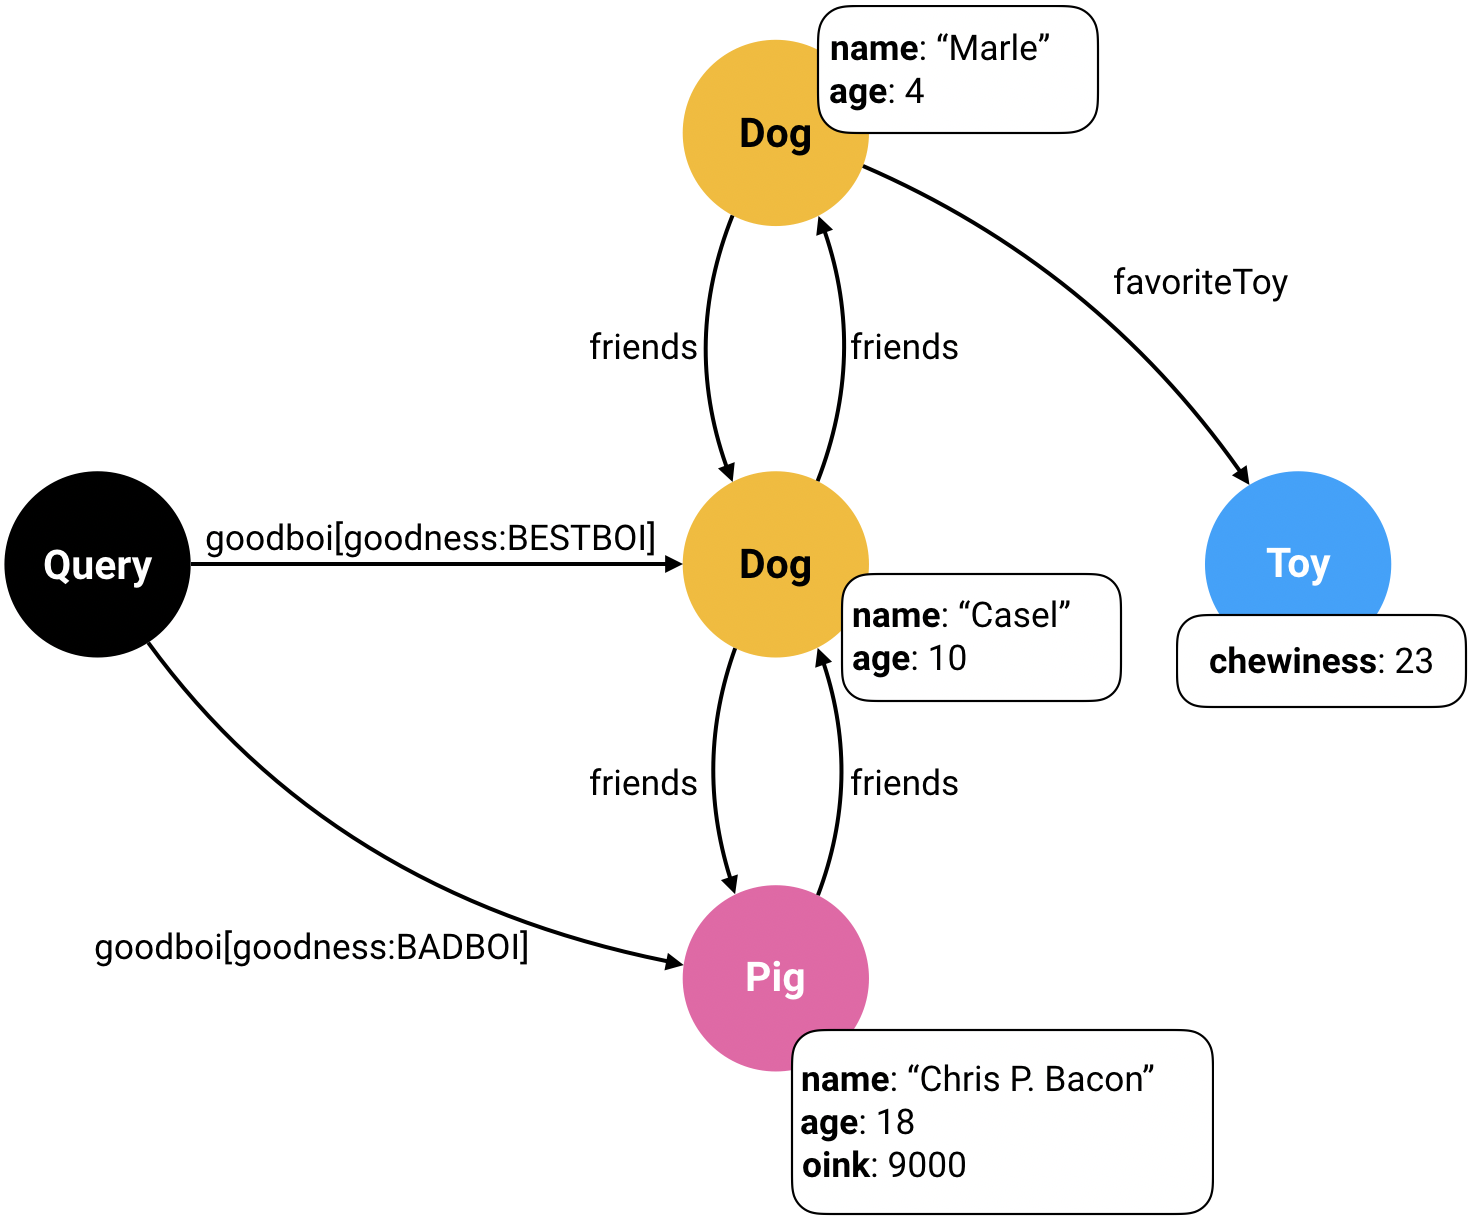
\includegraphics[scale=0.32]{imgs/graph.png}
    \caption{Example of \gql graph.}
    \label{fig:graph_ex}
\end{figure}

%Finally, now that we have defined our type system and data, our developers can proceed to query it.

%\fo{The following three paragraphs were moved from \S \ref{subsec:graph} and should
%be integrated into this section.} An important aspect of \gql is that it is not tied to any particular database technology and implementation. When resolving queries, \gql simply assumes the existence of \textit{resolvers}, which are internal functions defined by the user implementing a \gql service. They are not tied to any particular data model and the only requirement is that they must adhere to the schema. It is up to the user whether the resolvers access a database, return static values or even modify existing data\footnote{The \spec{} states that resolvers ``\textit{must always be side effect‐free and idempotent}'' but the definition of a resolver does not actually impose these restrictions.}. This looseness makes it hard to reason about the semantics.

%With this in mind, we choose to follow \HP's approach and define the underlying data model as a graph over which queries are evaluated. With this model, the unspecified resolvers can be instantiated to concrete definitions, which allow reasoning over them. The semantics are then described as being implemented over a graph setting. Although this provides benefits when reasoning about the semantics, it also comes with some potentially severe limitations over the completeness of the possible results generated.\td{They may not actually be limitations with the model, but there are open questions on how to model some things.} We provide a more thorough explanation of these in \S\ref{sec:discussion}, as well as \HP's approach to the subject.

%Informally, a \gql graph is a directed property graph, with labeled edges and typed nodes. The graph describes entities with their types and properties, as well as the relationship between them. This means that every node has properties (key-value pairs) and a type. Also, every label in an edge describes the relation between two nodes. Finally, every property or label may also contain a list of arguments (key-value pairs).


\paragraph{\gql query and response.}

With the schema and data defined, it is possible to query the service. 
As previously hinted, \gql queries are performed over the types and fields defined in the schema.
They have a tree structure, similar to \json, which follows the fields and relations established between the types
in the type system.

To illustrate this, we define the query in
Figure~\ref{fig:qres_ex}. Intuitively, we request the name of the best
animal in \goodbois, as well as the name and some additional
information of its friends. The query starts by selecting the field
\texttt{goodboi} of the \texttt{Query} type and providing the argument
\texttt{BESTBOI}. The type of this field is the interface
\texttt{Animal}, therefore the query continues selecting the field
\texttt{name}, with scalar type \texttt{String}, and the field
\texttt{friends}, with type \texttt{[Animal]}.  Because the {\em interface
type} \texttt{Animal} is implemented by two different {\em object types},
namely \texttt{Dog} and \texttt{Pig}, one can use more specific
selections to further specify the fields that should be requested for
each object type. 
This is achieved by the pair of selections (called {\em inline fragments})
\ifrag{Dog}{\texttt{ favoriteToy \{ chewiness \} }} and \ifrag{Pig}{
  \texttt{loudness:oink} }, which indicate that in the case of a 
dog, the query should request information about field
\texttt{favoriteToy}, while in the case of a pig, the query should
retrieve field \texttt{oink}. In this case, the field selection
\texttt{loudness:oink} is a {\em field alias}, which indicates that
the resulting value should be renamed to \texttt{loudness} in the response, instead of using the original field name \texttt{oink}.  
%\fo{Maybe introduce here ``inline
%  fragment'', ``selection'', etc.}

This query is then evaluated over the graph, resulting in the response
depicted on the right of Figure~\ref{fig:qres_ex}, whose structure closely
resembles the query.  The intuition behind the evaluation process is
that the query indicates what edges to traverse in the graph and what
properties to access on each node. In this manner, starting from the
node with type \texttt{Query}, the field \texttt{goodboi(goodness:
  BESTBOI)} indicates that the evaluation should continue in an
adjacent node reached after traversing an edge whose label matches the
field. The first step then takes the evaluation process to the central
node, of type \texttt{Dog}.  From there, the query accesses the value
of the node's property matching the field \texttt{name} and then
continues navigating the graph in search of the dog's friends.

%As previously mentioned, the queries we perform over our system must be over the types and fields defined in the schema. Every query must start by requesting information from the \texttt{Query} type. That means that, in our setting, queries must all start with the \texttt{goodness} or \texttt{search} fields.

%In figure \ref{fig:qres_ex}, we can see a query where we asking for all the friends of the \texttt{BESTBOI} in our system. For each friend we ask for their \texttt{name}. The query can be further specified, using fragments, and say that for the \texttt{Dog} friends we want to know their toy's \texttt{chewiness} and for the \texttt{Pig} friends, their \texttt{oink} level. We rename this last selection to \texttt{loudness}. As we can see from this example, queries in \gql have a tree structure similar to \json.

%If we evaluate this query in the graph depicted in \ref{fig:graph_ex}, we would get the response shown in figure \ref{fig:qres_ex}. This response was obtained by navigating the graph and collecting the information contained in each of the relevant nodes. It is easy to see that the response has a structure very similar to the query's.


\begin{figure}
\centering
\begin{subfigure}{.25\textwidth}
\begin{minted}[fontsize=\scriptsize, escapeinside=||,mathescape=true]{js}
query {
  artist(id: 1000) {
    name
    artworks(role: ACTOR) {
      title
      |$\ldots$| on Fiction {
        releaseYear:year
      }
      |$\ldots$| on Animation {
        style
      }
    }
  }
}

\end{minted}
\label{fig:query_ex}
\end{subfigure}%
\begin{subfigure}{.25\textwidth}
\begin{minted}[fontsize=\scriptsize]{json}
{
  "artist": {
    "name":"Tom Hanks",
    "artworks":[
      {
        "title": "Forrest Gump",
        "releaseYear": 1994
      },
      {
        "title": "Toy Story",
        "style": "3D"
      }
    ]
  }
}
\end{minted}
\label{fig:response_ex}
\end{subfigure}
\caption{\gql query (left) and its response (right).}
\label{fig:qres_ex}
\end{figure}

% \td{We can probably skip this paragraph to save space}
% As a final note, one of the appeals of \gql is that if we change our minds and no longer wish to request the friends's names, it would only suffice to remove the field selection 
% \texttt{name} from the \texttt{friends} subselections, and the generated response would no longer contain that piece of information. Similarly, reordering the output is simply done
% by reordering the selections in the query.
% We would not be required to define a new endpoint nor we would get
% information we no longer needed, as is usual the case with RESTful
% services. 


%If we wanted to ask another the same query but now without the friends' names, we would only have to remove the \texttt{name} field and \textit{voilà}, that's it. We use the same endpoint as before and the \gql service handles the resolution of our fields.

To summarize,
% This concludes our brief introduction to \gql and we can now move onto the formalization.
% The key points to take from our example are that 
in order to define a \gql service it is necessary to define the schema that describes the service's type system, 
to which both the underlying dataset and the queries must adhere. \gql queries consist of {\em selections} over fields and types defined in the schema, and their responses closely match the queries tree structure.

% !TEX root = ./main.tex
\section{\gcoql}\label{sec:form}

In this section we describe our formalization of \gql in \coq. We start by defining a schema and its properties, then the graph data model and finally we review queries and their semantics. The definitions are as close as possible with respect to the \spec. This eyeball correspondence between the definitions in prose and the code gives a first level of trust that our formalization is correct.%, following the examples of X, Y and Z.
Whenever there is a mismatch we point it out and explain the reasoning behind each decision.


\subsection{Schema}\label{subsec:schema}
We formalize schemas and type definitions following the \spec. A schema is represented as a record, containing a list of type definitions and a root type that specifies the available selections (\eg \texttt{Query} in the example from Figure \ref{fig:schema_ex}):
%

\begin{minted}[bgcolor=coqbg]{coq}
Record graphQLSchema := GraphQLSchema {
    query_type : Name;
    type_definitions : seq TypeDefinition }.
\end{minted}
%
Schemas may also include additional root types for specifying mutations and subscriptions (\cf\S3.2.1~\cite{gqlspec}). These operations are, however, out of the scope of our formalization.

Our formalization of type definitions closely follows the \spec, as
depicted in Figure~ \ref{fig:types_def}. A type may be a scalar type,
an object type, which possibly implements a set of interfaces, an
interface type, a union type or an enumeration type. Object and
interface type definitions comprise an (ordered) set of fields; union
types are defined by a set of type names and enumeration types by a
set of values. For the corresponding type definitions to be valid, all
such three sets should be non-empty. While the \spec enforces this
requirement syntactically (see the grammar on the left of Figure~\ref{fig:types_def}), we perform this validation when verifying the (overall) well-formedness schemas.     
%
\setlength{\grammarparsep}{10pt plus 1pt minus 1pt} % increase separation between rules
\begin{figure*}[h]
    \centering
    \begin{subfigure}{.5\textwidth}
    \begin{displaymath}
    \small
	\begin{array}{rl}
	\mathit{TypeDefinition} & ::= \\
	 | & \texttt{scalar } \name  \\
	 | & \texttt{type } \name\; (\texttt{implements } \name^{+})^{?} \texttt{ \{} \mathit{Field}^{+} \texttt{\}}\\
	 | & \texttt{interface } \name \texttt{ \{} \mathit{Field}^{+} \texttt{\}}\\
	 | & \texttt{union } \name \texttt{ = } \name\; (\texttt{|} \name)^{*}\\
	 | & \texttt{enum } \name \texttt{ \{} \name^{+} \texttt{\}} \\
	& \\
	\mathit{Field} & ::= \name \texttt{ (} \mathit{\overline{Arg}} \texttt{) : } \mathit{Type}\\
	& \\
    \mathit{Arg} & ::= \name \texttt{ : } \mathit{Type}\\
	& \\
    \mathit{Type} & ::=\\ 
     | & \name \\
 	 | &  \texttt{[}  \mathit{Type} \texttt{]}
	\end{array}
	\end{displaymath}
	
    
    %\fo{We may also want to use a less pompous grammar here}
    \end{subfigure}%
    \begin{subfigure}{.5\textwidth}
    \begin{minted}[bgcolor=coqbg]{coq}
    Inductive TypeDefinition : Type :=
    | ScalarTypeDefinition (name : Name)
    | ObjectTypeDefinition (name : Name)
                           (interfaces : seq Name)
                           (fields : seq FieldDefinition)
    | InterfaceTypeDefinition (name : Name)
                              (fields : seq FieldDefinition)
    | UnionTypeDefinition (name : Name)
                          (members : seq Name)
    | EnumTypeDefinition (name : Name)
                         (members : seq EnumValue).

    Inductive type : Type :=
    | NamedType : Name -> type
    | ListType : type -> type.
    \end{minted}

    \end{subfigure}
    \caption{Definition of \gql types: (left) \spec grammar; 
    (right) \gcoql definition.\newline
    {\footnotesize The $(\cdot)^{?}$ notation denotes optional attributes.}
    \td{Changed the optional bracket here also -- to $( )^{?}$}
    \td{Also changed $\overline{Field}$ bc the grammar specifies at least one}
    }
    % \fo{In the grammar, I would push the scalar case to a new line, to match the \coq snippet on the right} \et{done}
    \label{fig:types_def}
\end{figure*}


% As can be seen from the figure, our implementation looses information about non-emptiness of fields, union and enum members. We push this validation to a posterior predicate, as well as the discussion about the reasons behind this decision, to the following paragraphs.

% As can be seen in the figure, we tried to match the \spec's definition as much as possible. This eyeball correspondence gives us a degree of confidence about the implementation.  % We currently do not include the \textit{Input Object} types, as well as anything related to \textit{introspection}.

In this regard, observe that the provided definitions of schema and types allow building ``invalid'' schemas. For instance, one can build an object that implements scalar types or use a nonexistent type as the query type. To avoid this problem, the \spec provides several validation rules, scattered throughout the document (though most can be found in \S3~\cite{gqlspec} under each type description).
 % the \textbf{Type Validation} subsection of each type described in ..  
 We gather all these rules and refer to them as the \textit{well-formedness}
condition of a \gql schema:\footnote{In \HP, this notion is called {\em consistency}.}

\begin{definition}
A \gql schema is \textit{well-formed} if: 
\begin{itemize}
    \item its root type (is defined and) is an object type, 
    \item there are no duplicated type names, and
    \item every type definition is \textit{well-formed}.
\end{itemize}
\end{definition}

In \gcoql, this is captured by the Boolean predicate below. %As mentioned in the introduction, our formalization heavily relies on Boolean reflection, following the SSReflect mindset.
%
\begin{minted}[bgcolor=coqbg]{coq}
Definition is_a_wf_schema (s : graphQLSchema) : bool :=
      is_object_type s s.(query_type) &&
      uniq s.(schema_names) &&
      all is_a_wf_type_def s.(type_definitions).
\end{minted}
%
% \et{naming inconsistency between is\_a\_wf\_schema and is\_wf\_typedef: skip the "a" in the case of schema}
% \td{I had actually renamed it is\_a\_wf\_typedef. I prefer with the "a" tbh}
The notion of well-formedness for type definitions requires \eg that
union members contain existent object types and that object and
interface types contain at least one field. Due to space limitations,
we omit the full definition and refer the interested reader to our
\coq development. %file \texttt{SchemaWellFormedness.v}.

%We will, though, resume the discussion about non-emptiness of fields, union and enum members, which are included in the predicate. The main reason behind this decision is that, even though the \spec embeds this information in the grammar, it still includes it in their validation rules later on. We believe that it is simpler to use common lists instead of defining new structures or using dependent types, from an implementation point of view, while still preserving the correspondence to the algorithmic description given by the \spec.
%\td{Not sure if correctly worded... but it was just simpler to use lists. A non-empty list structure required coercions to lists and then redefining some lemmas and things. Or using dependent types (sigma type) adds complexity when proving and defining things (at least that was the case for me)}


% There are two main reasons why we push this rule to a separate predicate instead of embedding it in the structure itself. The first one is that, even though the \spec embeds it in the grammar, it still includes it in a validation rule later on. To match their definition and preserve the eyeball correspondence, we also include it. The second reason is that we use SSReflect and it is simpler to use \mintinline{coq}{seq} directly and all its theory, instead of defining coercions and repeating definitions for a new structure.

For convenience, we encapsulate schemas with their well-formedness
proof in a single structure. This structure also contains the
predicate \mintinline{coq}{is_a_valid_value}, which determines whether
a value used in a query indeed matches the scalar type expected by the
schema. For example, if a field argument has type \texttt{Float}, the
\spec requires that the actual argument used in a query represent a double-precision fractional value\footnote{The \spec declares a set of minimal scalar values and how they should be represented, such as floating-point values adhering to IEEE 754. We do not include this base restrictions but leave it open to implementation.}.
%
\begin{minted}[bgcolor=coqbg]{coq}
Record wfGraphQLSchema := WFGraphQLSchema {
    schema : graphQLSchema;
    _ : schema.(is_a_wf_schema);
    is_a_valid_value : type -> Vals -> bool; }.
\end{minted}

%\fo{Mention what \texttt{Vals} represents (used here for the first
%  time, but not defined)}


% This predicate is necessary to establish when a value used in a query or in the graph actually matches the scalar type expected by the schema. For instance, if an argument requires a \texttt{Float} value, then the actual value passed to the query must be something that represents a double-precision fractional value\footnote{The \spec declares a set of minimal scalar values and how they should be represented, such as floating-point values adhering to IEEE 754. We do not include this base restrictions but leave it open to implementation.}. This predicate validates that this is satisfied.

% Due to space constraints, we omit the definition of \textit{well-formedness} for type definitions. This property includes things such as: interfaces and objects must declare at least one field, objects correctly implement their declared interfaces, union types are not empty and contain only object types, amongst others. These definitions are collected from the \spec \td{Scattered throughout the \spec*}.

Having reviewed our formalization of schemas, we now discuss our formalization of the data model. 



\subsection{Data Model}\label{subsec:graph}
Following \HP, we adopt a data model based on graphs, where data are
modeled as directed property graph, with labeled edges and typed
nodes. Nodes contain a type and a set of properties (key-value pairs)
and  edges contain single labels that describe the relations between
adjacent nodes. Also, every property and label may contain a list of
arguments (key-value pairs). %Refer to Figure~\ref{fig:graph_ex} for an example.

To represent the values associated to properties and arguments, we consider the type \Vals. 
% A value in \Vals may be a single scalar value or a list of values\td{This choice is based on the limitations of the model}.\fo{I think we should address this in the Discussion section, where we discuss the limitations of our formalization. We could even remove the last sentence from the paragraph.}

\begin{definition}
A \emph{\gql graph} over \Vals{} is defined by:
\begin{itemize}
    \item a root node, and
    \item a collection of edges of the form ($u$, $\fld$, $v$), where $u, v$ are nodes and
      $\fld$ is a label with arguments
      (key-value pairs).
\end{itemize}
\end{definition}

In \gcoql, this is captured by the following structures. 
% A \texttt{label} represents the set of labels over an edge or keys in a node's property. 
%\td{Probably the name is not the best}\fo{Fully agree. I suggest changing \texttt{fld} to \texttt{label}, \texttt{Field} to \texttt{Label} and \texttt{label} to \texttt{name} (or \texttt{lname} if there is a clash) }. 
%
\begin{minted}[bgcolor=coqbg]{coq}
Record label := 
  Label { lname : string; args : seq (string * Vals) }.

Record node := 
  Node { ntype : Name; nprops : seq (label * Vals) }.

Record graphQLGraph := 
  GraphQLGraph { root : node; 
                 edges : seq (node * label * node) }.
\end{minted}
The root node of a \gql graph represents the starting point from where queries are evaluated. Note that edges are modeled as a list, and not as a set; unicity of its members is handled by a separate validation. 
 % and include a posterior separate validation on uniqueness of its members.
This found this approach more convenient in the current development, but this design decision would be fairly easy to revisit if needed.
% \td{Added this}


Intuitively, the data modeled by a \gql graph is expected to respect
(the type system described by) a schema. However, the definition of
graphs above is fully independent of schemas. To relate the data to the type system, we define the notion of \textit{conformance} of a graph \wrt a schema, partially based on~\cite{gqlph}.
%
\begin{definition}
A \gql graph $\mathcal{G}$ \textit{conforms} to a schema $\mathcal{S}$ if:
\begin{itemize}
    \item the types of $\mathcal{G}$ root node and $\mathcal{S}$ query
      root coincide,
    \item every node of $\mathcal{G}$ \textit{conforms} to
      $\mathcal{S}$, and
    \item every edge of $\mathcal{G}$ \textit{conforms} to
      $\mathcal{S}$. 
   
\end{itemize}
\end{definition}
%


The conformance of nodes includes rules such as checking that a node
type is declared as an object type in the schema and that its
properties are defined as fields in the corresponding type. Among
others, the conformance of edges ensures that edge labels are declared
as a field in the source node's type and the target node has a type
compatible with the field's return type. Full definitions of both
these notions can be found in the \coq development. %are found in file \texttt{GraphConformance.v}.

With this in mind, the notion of conformance of a graph \wrt a schema is formalized as follows:
%
\begin{minted}[bgcolor=coqbg]{coq}
Definition is_a_conforming_graph 
      (s : wfGraphQLSchema) (g : graphQLGraph) : bool :=
  root_type_conforms s g.(root) &&
  edges_conform s g &&
  nodes_conform s g.(nodes).
\end{minted}
%
% As a side note, this notion was only loosely defined in \HP, but it is properly addressed in a recent work of one of its authors ~\cite{olafschema}.

Similarly to \gql schemas, we define a structure that encapsulates the notion of a \textit{conformed} graph, containing a graph and a proof of its conformance to a particular schema.

\begin{minted}[bgcolor=coqbg]{coq}
Record conformedGraph (s : wfGraphQLSchema) :=
  ConformedGraph { graph : graphQLGraph;
                       _ : is_a_conforming_graph s graph }.
\end{minted}

 %These properties include validation rules such as: every node must have an object type and their properties must be defined in their associated type, or an edge's label must be declared as a field in the source node's type and the target node must have a type compatible to the field's return type, among other things.

%With both the schema and the underlying data model we can proceed to define \gql queries and their semantics.


\subsection{Queries}\label{subsec:query}
To define queries we faithfully follow the \spec, as shown in
Figure~\ref{fig:query_def}. A query consists of a list of selections, and can optionally be named.
% consists of an optional name
% \fo{We should mention this also in \S 2}\td{Not really necessary, or is it?} and a list of selections. 
A selection $\sel$ can be a single field $\fld$ with arguments, an aliased field $\afld$, or a possibly-aliased field followed by a set of subselections $\sset$, or an inline fragment $\ifrag{t}{\sset}$ comprising a type condition \texttt{t} and a set of subselections $\sset$. 
% Fields can be accompanied by a list of arguments and can also be renamed.

\begin{figure*}[h]
  \centering
  \begin{subfigure}{.5\textwidth}
  \begin{displaymath}
	\begin{array}{rcl}
	\query & ::= & \texttt{query } (\name)^{?} \texttt{ \{}  \sset \texttt{\}} \\
	&& \\
	\sel & ::= & \fld \\
	& | & \afld \\		
	& | & \nfld{\sset} \\
	& | & \anfld{\sset} \\
	& | & \ifrag{t}{\sset} \\
	\end{array}
	\end{displaymath}
	
	\iffalse
    \begin{grammar}
    		<Query> ::= [\textbf{\texttt{query}} [<name>]] \textbf{\texttt{\{}} <Selection>$^{+}$ \textbf{\texttt{\}}}
		
        <Selection> ::= <name> \textbf{\texttt{(}} <Arg>* \textbf{\texttt{)}}
        \alt <alias> \textbf{\texttt{:}} <name> [\textbf{\texttt{(}} <Arg>$^{+}$ \textbf{\texttt{)}}]
        \alt <name> [\textbf{\texttt{(}} <Arg>$^{+}$ \textbf{\texttt{)}}] \textbf{\texttt{\{}} <Selection>$^{+}$ \textbf{\texttt{\}}}
        \alt <alias> \textbf{\texttt{:}} <name> [\textbf{\texttt{(}} <Arg>$^{+}$ \textbf{\texttt{)}}] \textbf{\texttt{\{}} <Selection>$^{+}$ \textbf{\texttt{\}}}
        \alt \textbf{\texttt{... on}} <name> \textbf{\texttt{\{}} <Selection>$^{+}$ \textbf{\texttt{\}}}
        
        <Arg> ::= <name> \textbf{\texttt{:}} <value>
    \end{grammar}
    \fi 
    
  \end{subfigure}%
  \begin{subfigure}{.5\textwidth}

    \begin{minted}[bgcolor=coqbg]{coq}
    
    Record query := 
         Query { qname : option string; 
                 selection_set : seq Selection }.
                   
    Inductive Selection : Type :=
    | SingleField (name : Name)
                  (arguments : seq (Name * Vals))
    | SingleAliasedField (alias : Name)
                         (name : Name)
                         (arguments : seq (Name * Vals))
    | NestedField (name : Name)
                  (arguments : seq (Name * Vals))
                  (subselections : seq Selection)
    | NestedAliasedField (alias : Name)
                         (name : Name)
                         (arguments : seq (Name * Vals))
                         (subselections : seq Selection)
    | InlineFragment (type_condition : Name)
                     (subselections : seq Selection).
    \end{minted}
  \end{subfigure}
  \caption{Definition of \gql queries:
  (left) \spec grammar; 
  (right) \gcoql definition.
  \newline{\footnotesize Symbols \texttt{f}, \texttt{a} and \texttt{t} correspond to identifiers for field names, field aliases and type conditions, respectively.
  Symbol $\args$ stands for a list of key-value pairs, representing the arguments of fields.}
  %\td{Brackets in optional query name may conflict with the others? It is a diff font, but idk if maybe using something else=}
  %\et{yeah that's a bit unfortunate. A solution is to use $( ... )^?$ to denote optional elements (without parenthesis when it's a single element)}
  %\td{Is it me or the query record looks flattened?} \et{???}
  } %\td{To be completely accurate, the parenthesis in field selections are not necessary unless there are arguments}\td{This might add some noise?}\et{yeah I think that'd be too much (and not very relevant)}
  \label{fig:query_def}
\end{figure*}

Intuitively, a valid query and its selection set form a tree, where leaves correspond to fields of scalar types and inner nodes correspond either to fields of some object type or abstract type (\ie~interface or union),
% \fo{abstract type not defined}\td{Ok like this?} 
or to inline fragments that condition when their subselections are evaluated. 

\iffalse
%For instance, the query in Figure \ref{fig:qres_ex} can be depicted as the tree in Figure \ref{fig:query_tree}.
\begin{figure}
    \centering
    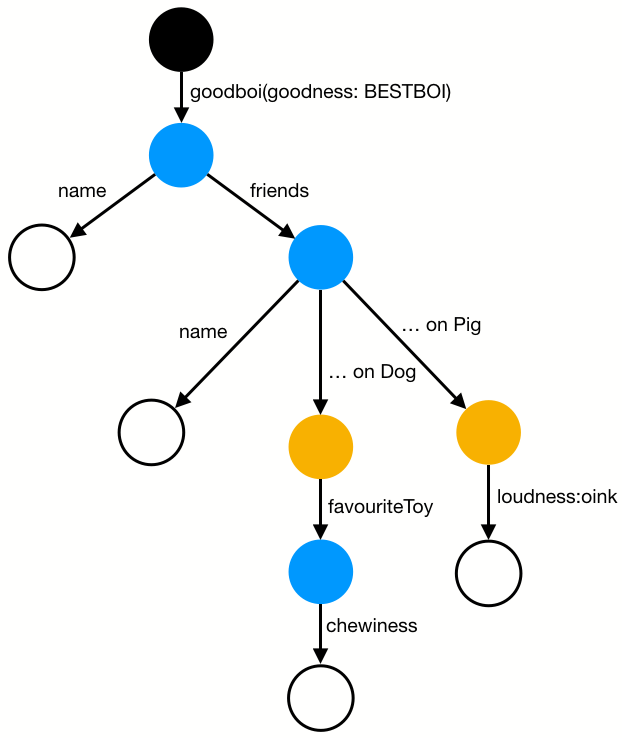
\includegraphics[scale=0.33]{imgs/query_tree.png}
    \caption{\gql query as a tree.}
    \label{fig:query_tree}
\end{figure}
\fi 

% Similar to the schema definition, we follow the \spec's grammar as closely as possible, as can be seen from Figure~\ref{fig:query_def}. We do not embed the property of non-emptiness of subqueries in the definition because the \spec pushes it to a different validation rule, even though it is already embedded in the grammar, and we believe it is simpler to reuse the \texttt{seq} library and its existent functionalities. 

Observe that the definition of queries in Figure~\ref{fig:query_def}
is not bound to any schema, requiring thus a separate validation
process to ensure that they adhere to a given schema. We introduce the
notion of query \textit{conformance}, based on a set of validation
rules scattered throughout the \spec (\cf\S5~\cite{gqlspec}). The
validity of queries depends on the validity of their selection sets,
which in turn requires the notion of \textit{type in context} at a
given selection location\footnote{The \spec refers to it as the \emph{type in scope} or \emph{parent type}. Some algorithmic descriptions make use of the types in context but are not explicit in their signatures.}. % Since queries are selections over the fields of types, it is important to know exactly to what type they are being applied.
To illustrate this, consider the following query with two occurrences of field \texttt{name}.

%\begin{minipage}[t]{.25\textwidth}
\begin{minted}[escapeinside=||, mathescape=true]{js}
query {
  goodboi {
    |$\ldots$| on Dog {
      name
      favoriteToy
    }
    |$\ldots$| on Pig {
      name
      favoriteToy
    } } }
\end{minted}
%\end{minipage}%
% \begin{minipage}[t]{.25\textwidth}
% \begin{minted}[escapeinside=||, mathescape=true]{js}   
% type Human {
%   age: Int
% }

% type Martian {
%   age: Float
% }
% \end{minted}
% \end{minipage}
%\et{for space reason, we may want to take some liberties wrt the formatting of queries and responses (see some examples on this page)}


\noindent In the first occurrence, the field is requesting information about the
\texttt{Dog} type, while in the second it is requesting information about the \texttt{Pig} type. The distinction is important because some field selections might be valid in some contexts but not in others. This is the case, for instance, for field \texttt{favoriteToy}: It is valid in the context of a \texttt{Dog} type but it is invalid in the context of a \texttt{Pig} type, as \texttt{Pig} type does not contain any such field. %Similarly, the above query would also be invalid if \texttt{Pig} type contained a so-called field, but of type different from \texttt{Toy} ---the type of the same field in type \texttt{Dog}.

%Just as in the case of well-formedness of schemas or conformance of graphs, queries must go through a validation process. We define the property of \textit{conformance} of queries, based on validation rules scattered throughout the \textit{Validation} section of the \spec\footnote{https://graphql.github.io/graphql-spec/June2018/\#sec-Validation}.

% Before describing the validation process, it is very important to address the notion of \textit{type in context} where queries are defined and used. The type in context is the type over which a user might be requesting information on its fields. To illustrate this, consider the following query. The first selection, namely \texttt{goodboi}, is requesting information about the query type, meaning that it is used in the context of the \texttt{Query} type. Moving onto the  \texttt{name} subselection, it is not direct which is. In one case, the type in context is \texttt{Dog}, while in the other the field is used in the context of the \texttt{Pig} type.

% The importance of this type in context is that fields or inline fragments might be valid in certain cases but not in others. Similarly, a field may have a particular return type in one case and a different one in another type, like in the following example. Both types have an \texttt{age} field, but in one case it returns an integer value while in the other a floating point value. If that field is encountered in a query, it is necessary to know to which type it is being requested.

Now that we have clarified the notion of type in context, we are in
condition of defining the notion of query conformance, which in turn
depends on the notion of selection set conformance.

%\td{A query conforms when its selections conform to the Query type}
\begin{definition}
A \gql selection set $\sset$ \textit{conforms} to a schema $\schema$ over a type in context $\mathit{ts}$ if:
\begin{itemize}
\item every selection in $\sset$ is  well-formed, and

\item any two field selections in $\sset$ are type-compatible and
  renaming-consistent\footnote{In the \spec
    (\cf\S5.3.2~\cite{gqlspec}), these two notions roughly correspond
    to \emph{having-the-same-response-shape} and
    \emph{fields-can-merge}, respectively.}.
       
\end{itemize}
\end{definition}

The first rule ensures that every selection is well-formed on its own, with
respect to the type in context. Its requirements vary according to the
kind of selection. For instance, if the selection is a field, the rule
checks that the field is part of the type in context and that its
arguments are correctly provided; if the selection is an inline
fragment, then the type condition must at least share one subtype with
the type in context.


In the second rule, the type-compatibility requirement forbids the
selection set in \eg the following query:

\begin{minipage}[t]{.22\textwidth}
\begin{minted}[escapeinside=||,mathescape=true]{js}
query {
  goodboi {
    friends {
      |$\ldots$| on Dog {
        name
     }
     |$\ldots$| on Pig {
       name:oink
} } } }
\end{minted}
\end{minipage}%
\begin{minipage}[t]{.22\textwidth}
\begin{minted}[escapeinside=||,mathescape=true]{js}
// Possible invalid output
{
  "goodboi" : {
       "friends" : [
         { "name" : "Marle" },
         { "name" : 9000 }
     ]
} }
\end{minted}
\end{minipage}

Intuitively, the previous query is invalid because its evaluation can produce results with the same key 
(key \texttt{name}) but associated to values of different type (string and integer values).

%\td{We are not exactly capturing that the fields can be inside fragments, is it ok?}\et{I don't get it}
The definition of field \emph{type-compatibility} is recursive. Two nested
field selections are type-compatible if whenever
they have the same response name, any two fields in the concatenation of their
subselections are also type-compatible. Two single field selections
are always type-compatible, unless they have the same response
name and different (scalar or enum) type.

Finally, the renaming-consistency condition ensures that fields with
the same response name refer to the same piece of information. For
instance:
% \td{This leaves a lot of empty space :/}
\begin{minted}[escapeinside=||,mathescape=true]{js}
query { goodboi {
          age   
          |$\ldots$| on Pig { age:oink } }
\end{minted}

Intuitively, this query is considered invalid because the fields with response name \texttt{age} both refer to distinct pieces of information;
the first occurrence refers to the age of the animal, while the second accesses the field \texttt{oink} but renames it accordingly.

%\fo{Add example and briefly explain} 

Two field selections are \emph{renaming-consistent} if whenever they have the
same response name and lie under overlapping types in context
\fo{@Eric, is there any standard terminology for this
  ``overlapping'', meaning that they share at least one subtype?},
  \et{sharing a subtype means that their "(subtyping) meet/glb" exists--is that what you're referring to?}
  \td{Yeah, at least I believe it is}
they have the same (actual) name, the same arguments and any two
fields in the concatenation of their subselections are also
renaming-consistent.

The last two rules are defined as a single validation rule in the \spec (\cf\S5.3.2~\cite{gqlspec}). 
We choose to split them because we noticed that they indeed can be defined separately, simplifying their implementation as well as facilitating 
reasoning about them\footnote{Our algorithm implements an optimized version of the rule. A team at XING\footnote{https://www.xing.com/} recently published another algorithm described in~\cite{xingalg}.}.


\begin{definition}
A \gql query $\query$ \textit{conforms} to a schema $\schema$ if its selection set conforms to $\schema$ over the query root type.
\end{definition}

%\et{this is the beginning of the problem I'm having with your statements about queries. There is the notion of *a query*, noted $\varphi$, yet from now on your statements are about *queries*. The definition below mixes "the content" (consistency, compatible response, etc.) with "the sequence" (all, list comprehension, etc). Worse, later on in the development, you use $\varphi$ as the variable name of type "seq Queries" (while fig6 uses a bar over). See also my later comments about your "plural formulations"}

\noindent In \gcoql, this is captured with the following predicates.

%The implementation can be seen in the code below, however due to space limitations we only informally describe the %three mentioned rules. The complete definitions can be found in the file \texttt{QueryConformance.v}.

\begin{minted}[bgcolor=coqbg, escapeinside=@@, mathescape=true]{coq}
Definition query_conforms 
    (s : wfGraphQLSchema) (@$\query$@ : query) : bool :=
    selections_conform s s.(query_type) @$\query$@.(selection_set).
    
Definition selections_conform (s : wfGraphQLSchema)
    (ts : Name) (@$\sel$@s : seq Selection) : bool :=
        all (is_consistent ts) @$\sel$@s &&
        is_field_merging_possible ts @$\sel$@s &&
        have_compatible_response_shapes
            [seq (ts, @$\sel$@) | @$\sel$@ <- @$\sel$@s].

\end{minted}

% This concludes the definition of \gql queries, the validation process and the notion of size of selections. 
From now on, it is assumed that queries conform to a given schema. Finally, most of the recursive definitions over selection sets are well-founded using a notion of size.
\begin{definition}[adapted from \cite{gqlph}]
% \td{It is in essence the same, except that they define selections along with queries}
The \emph{size} of a selection $\sel$ and selection set $\sset$, noted $\ssize{\cdot}$, is recursively defined as:
\begin{small}
\begin{align*}
    \ssize{\fld}  = \ssize{\afld} &=  1\\
    \ssize{\nfld{\sset}} = \ssize{\anfld{\sset}} = \ssize{\ifrag{t}{\sset}} &= 1 + \ssize{\sset}\\
    \ssize{\sset} &= \sum_{\sel_{i} \in\; \sset}{\ssize{\sel_{i}}}
    \end{align*}
\end{small}
\end{definition} 

%\td{Cannot define $\sset$ in Coq (lexer error), so I had to go with $\sel$ instead of the selection set and simply \texttt{sel} for an atomic selection}
 %\et{you can use "$\sel$s"}
%\fo{This introduces the conformance of a query \wrt a schema, but the schema is never mentioned in the definition. It needs to be fixed!!!}


%has to be valid with respect to the type in context \fo{when can it not be valid?}\td{If both the type condition and the type in context do not share at least one subtype (subtype is reflexive). Not sure if this is relevant here though}.%The \spec defines this rule in several different sections.

% The second rule validates when fields can be correctly merged during evaluation, which is an essential aspect of the semantics, since it ensures that repeated fields are only evaluated once. To illustrate this, consider the following query, where a user requests information on the fields \texttt{name} and \texttt{oink} of pigs. The user decides to rename the field \texttt{oink} to \texttt{name}, however this is invalid, since both fields cannot be merged and evaluated once; both fields refer to distinct pieces of information in the system.

% \begin{minted}[escapeinside=||,mathescape=true]{js}
% query {
%   goodboi {
%     name    
%     |$\ldots$| on Pig {
%       name
%       toy:oink
%     }
%     |$\ldots$| on Dog {
%       name
%       toy:age
%       }
% } } }
% \end{minted}

% The last rule is necessary to check when fields generate consistent values when evaluated. For instance, in the query below a user might request the names of dogs and the oinkness of pigs, but renaming the latter to have the same response name as the former. This query is considered invalid because evaluating it might produce a response that contains entries where the key \texttt{name} is associated to both string values and floating point numbers. 

% \begin{minipage}[t]{.22\textwidth}
% \begin{minted}[escapeinside=||,mathescape=true]{js}
% query {
%   goodboi {
%     friends {
%       |$\ldots$| on Dog {
%         name
%       }
%       |$\ldots$| on Pig {
%         name:oink
% } } } }
% \end{minted}
% \end{minipage}%
% \begin{minipage}[t]{.22\textwidth}
% \begin{minted}[escapeinside=||,mathescape=true]{js}
% // Possible invalid output
% {
%   "goodboi" : {
%     "friends" : [
%         { "name" : "Marle" },
%         { "name" : 9000 }
%     ]
% } }
% \end{minted}
% \end{minipage}




% The main issue is that the \spec allows for what we call \textit{invalid fragments}, originally described in an issue in the \spec's repository\footnote{https://github.com/graphql/graphql-spec/issues/367}. In a nutshell, the \spec allows using fragments with type conditions that can span to multiple unrelated types. These end up not being evaluated due to posterior checks\footnote{https://graphql.github.io/graphql-spec/June2018/\#DoesFragmentTypeApply()}.


% \td{This looks a bit weird... Should it be a "definition" or just inline it as \HP does?}





\subsection{Semantics}\label{subsec:semantics}
Now we have all the prerequisites to define the semantics of \gql queries and their selection sets. We begin by briefly examining the responses generated by executing queries and then we give an informal description of the semantics, finishing with the formal definition. %We finish by discussing some implementation choices and comparison with the \spec and \HP.

A first observation we need to make is that query semantics is not compositional, in the sense that the result of a sequence of selections is not obtained by concatenating the results of the individual selections. Therefore, our semantic function will take a (whole) sequence of selections and return a (whole) sequence of responses.  

We model responses with a tree structure, similar to JSON, as shown in Figure~\ref{fig:response_def}. A response can be a value, an object mapping keys to other responses or an array of response values. Null values in the leaves of the response tree are represented with option types.%\et{fix once fig 6 defs is clarified}


\begin{figure*}[h]
\centering
\begin{subfigure}{.5\textwidth}

  \begin{displaymath}
	\begin{array}{rcl}
	\response & ::= & \texttt{v}\\
	& | & \texttt{\{} (\fkey : \response) \ldots (\fkey : \response) \texttt{\}} \\
	& | & \texttt{[} \response \ldots \response \texttt{]}
	\end{array}
	\end{displaymath}
	
	
\iffalse
    \begin{grammar}
    		<ResponseValue> ::= <value>
		\alt \textbf{\texttt{\{}} (<name> \textbf{\texttt{:}} <ResponseValue>)* \textbf{\texttt{\}}}
		\alt  \textbf{\texttt{[}} <ResponseValue>* \textbf{\texttt{]}}
 \end{grammar}
 \fi
 
  \end{subfigure}%
  \begin{subfigure}{.5\textwidth}
\begin{minted}[bgcolor=coqbg]{coq}
Inductive ResponseValue (A : Type) : Type :=
| Leaf : A -> ResponseValue
| Object : seq (Name * ResponseValue) -> ResponseValue
| Array : seq ResponseValue -> ResponseValue.

Definition GraphQLResponse (Vals: eqType) :=
    seq (Name * (@ResponseValue (option Vals))).
\end{minted}
   
  \end{subfigure}
  \caption{Definition of \gql responses, the grammar matching JSON (left) and the \coq implementation (right).
   \newline{\footnotesize The keywords \texttt{v} and \fkey represent leaf values and keys in a key-value pair, respectively.}
  }
  \label{fig:response_def}

\end{figure*}
%

%\fo{What is the role of \texttt{ArrayResponse}? When presenting our domain of values \textit{Vals} you mentioned that it can be a scalar value, or a ``list'' of values. Is the \texttt{ArrayResponse} the counterpart of this ``list''? }

%\fo{Explain the role of each constructor}
%\fo{Shouldn't the ObjectResponse constructor take a GraphQLResponse argument?}



%\begin{figure}[h]

%\caption{Implementation in Coq of \gql responses.}
%\label{fig:responses}
%\end{figure}



% As we described in \S\ref{subsec:graph}, the underlying data model we use is a graph, therefore the semantics are instantiated to this setting. %In a following paragraph we briefly explore an alternative that is closer to the \spec, in the sense that it can be detached from a particular data model. 
\td{Maybe merge this informal description with the description of the figure?}
\et{yes}
Informally, the evaluation of a query's selection set represents a navigation over a graph, starting from the root node, traversing its edges and collecting data from its nodes. In this sense:
\begin{itemize}
    \item A field selection represents either accessing a node's property or traversing an edge to a neighboring node.
    \item An inline fragment conditions whether using a node to access its properties or to traverse to other nodes.
    \item Subselections are evaluations over neighboring nodes.
\end{itemize}

\begin{definition}
Let $\graph$ be a graph and $\sset$ a selection set, both conforming to a schema $\mathcal{S}$. The evaluation of $\sset$ over $\graph$ from node $u \in \mathit{nodes}(\graph)$\footnote{Where $\mathit{nodes}$ is a function that retrieves all nodes from a graph.}, denoted $\llbracket \sset \rrbracket^{u}_{\graph}$, is defined recursively as shown in Figure~\ref{fig:semantics}. 
\end{definition}

The definition starts with the base case of empty selection set, which results in an empty response (1). 
Single fields correspond to accessing a node's property that matches the field name (2). 
As specified in \spec (\cf\S6.4.3~\cite{gqlspec}), scalar values must be coerced and verified to match the scalar type expected by the schema, otherwise the value is considered null.
We model this with the function  $\mathit{coerce} : \mathit{Vals} \to \mathit{ResponseValue}$
\et{this is weird, I would have expected coerce to return an option, since you said earlier that possible null values are modeled with options}
\td{Aja! Yep, it actually is (ResponseValue (option Vals))}
\td{We build a wfCoercion by proving that the coerced value is not redundant -- this might need more explanation}.
On the other hand, nested fields (equation 3) represent a traversal to neighboring nodes. The semantics searches for nodes that are connected by an edge whose label matches the field name
and then evaluates the subselections on these nodes. If the field's type is not a list type, then the semantics should be able to at least traverse to a single neighboring node, otherwise the result is considered null. 
In both field cases, the evaluation process has to ensure that selections with the same response name are only evaluated once. 
This is performed by calling the $\mathit{collect}$, $\mathit{merge}$ and $\mathit{filter}$ functions, which respectively gather fields sharing the same response name, merge their subselections 
and remove their repeated occurrences. 
Finally, inline fragments simply condition whether their subselections should be evaluated in the current node. 
The decision is based on the $\mathit{fragment\_type\_applies}$ predicate that verifies whether the type condition is the same or a super type of the node's type\footnote{Aliased fields are not included since they are evaluated the same way as unaliased fields, but differ in that the key-value pair produced is renamed accordingly.}.

%The definition of the evaluation function for selections, displayed in Figure~\ref{fig:semantics}, only refers to the base case of an empty list, field selections without renaming and inline fragments. The complete definition can be found in the file \texttt{QuerySemantics.v}.

\begin{definition}
Let $\graph$ be a graph and $\query$ a query containing a selection set $\sset$, both conforming to a schema $\schema$. The semantics of $\query$ over $\graph$ is defined as the result of evaluating $\sset$ from the root node of $\graph$.
\end{definition}

The semantics of queries is then formalized as follows:
\begin{minted}[bgcolor=coqbg, escapeinside=||, mathescape=true]{coq}
Definition execute_query (s : wfGraphQLSchema)
    (g : conformedGraph s) (|$\varphi$| : query) :=
    execute_selection_set s g.(root) |$\varphi$|.(selection_set).
\end{minted}

%The formal definition of the semantics is depicted in Figure \ref{fig:semantics}. The definition displays the cases where a field selection is accessing a node's property, when it is navigating to other nodes and when it is evaluating an inline fragment. Aliased fields are omitted for brevity but the complete definition can be explored in the file \texttt{QuerySemantics.v}.




%\td{Don't know how to present this or if it is relevant but I include it so you know it exists - The spec first groups fields by name and then evaluates each group. These are different steps. We define everything in one place because it was easier to reason about the semantics. The difficulty with the spec's approach is that when proving things about the semantics, you have to provide, at each step, the information on how your data is structured (every group contains only fields and every field in a group has the same response name as the group's key used to group them). This is problematic mostly because of inline fragments, which do not have response names. Definitions must always account for the case of inline fragments, even when they are thought out to be used only on fields. Our definition is maybe less compositional but thanks to Equations, it is simpler to reason about it - because Equations generate a nice reasoning principle. We also attempted defining it similarly to the spec, still preserving the information on the structure by using dependent types and Equation, but the resulting reasoning principle would end up being huge (80-100 cases) (I believe I read Matthieu saying that nesting some definitions could exponentially increase the size of the reasoning principle, which is what would occur in this case).}


%Our first attempt at defining the semantics was to follow \HP's post-processing approach. Our intention was to be as close as possible to their formalization to later prove their transformation and equivalence results, which we cover in Section~\ref{sec:norm}. However, the non-structural recursive nature of both the transformations and the post-processing function made reasoning about semantic equivalence very hard.

\begin{figure*}[t]
\small
    \centering
    \begin{align*}
    % Empty
    & (1) & \eval{\cdot}{u} &= [\cdot] \\
    % SingleField
    & (2) & \evalu{\fld :: \sset} &= \begin{cases}
        \resp{\mathit{coerce(\val)}} :: \evalfilteru{\sset}{\fkey}  
        & \text{if } \mathit{property}_{u}(\fld) = \val \text{ and } \mathit{is\_valid\_response}(\mathit{coerce}(\val)) \\
        \resp{\nval} :: \evalfilteru{\sset}{\fkey} 
        & \text{otherwise}
    \end{cases}\\
    % Nested field
    & (3) & \evalu{\nfld{\overline{\beta}} :: \sset} &=
    \begin{cases}
        \resp{\texttt{[} \mathit{map}\; (\lambda v_{i}.\; \eval{\overline{\beta} \mdoubleplus \mathit{merge} (\mathit{collect}_{\fkey} (\sset))}{v_{i}})\; \mathit{neighbors}_{\fld}(u) \texttt{]}} :: \evalfilteru{\sset}{\fkey} \\  
         \hfill \text{ if } 
            \mathit{ftype_{type(u)}(\fkey)} = L \text{ and } \{v_{1}, \ldots, v_{k}\} = 
        \{v_{i} \mid (u, \fkey[\alpha], v_{i}) \in \mathit{edges}(\graph)\} \\
        %
    \fkey:\{\eval{\subqueries{\beta}}{v}\} ::  \evalfilteru{\sset}{\fkey}  
         \hfill \text{ if } 
        \mathit{ftype_{type(u)}(\fkey)}  \neq L \text{ and } (u, \fkey[\alpha], v) \in \mathit{edges}(\graph) \\
    %
    \resp{\nval} :: \evalfilteru{\sset}{\fkey} 
    \qquad \qquad \qquad \qquad \qquad
  \text{ if } \mathit{ftype_{type(u)}(\fkey)}  \neq L  \text{ and } \nexists v \text{ s.t. }  (u, \fkey[\alpha], v) \in \mathit{edges}(\graph) \\
    \end{cases}\\
    %inline fragment
    & (4) & \evalu{\ifrag{t}{\overline{\beta}} :: \sset} &= 
    \begin{cases}
    \evalu{\overline{\beta} \mdoubleplus \sset} 
     & \text{ if }\mathit{fragment\_type\_applies_{type(u)}(\texttt{t})}\\
    \evalu{\sset} 
    & \text{ otherwise}
    \end{cases}
    \end{align*}
    \caption{Semantics of \gql selection sets, adapted from~\cite{gqlph} and the \spec. 
    \newline {\footnotesize 
    $\mathit{property}$ and $\mathit{type}$ are accessors to a node's property and type. $\mathit{neighbors}$ gets the neighbors of a node whose edge is labeled with the given field.
    $\mathit{edges}$ gets the set of edges of a graph.  $\mathit{is\_valid\_response}$ validates the coerced value.
    $\mathit{ftype}$ retrieves the field's type in the schema. $L$ represents the list type.}}
    %The $\mathit{property}$ function is an accessor to a node's property value. The $\mathit{filter}$ function removes all fields with the given response name, while $\mathit{collect}$ gathers all fields that match the given response name. 
    %Meanwhile, $\mathit{merge}$ joins the subqueries of the input selections. The $\mathit{type}$ function retrieves the type of the given field in the node's type.
	%The $\mathit{fragment\_type\_applies}$ predicate checks if the fragment's type condition is related to the node's type and whether its contents should be evaluated in the given node.
	%Finally, $E$ are the graph's edges, while $L_{t}$ is simply the list type.
	% \et{then why the $_t$ subscript?}\td{Simply bc its "List type" -- I took the same notation as in \HP to somehow show the similarity between both definitions.}\et{remove it, it's confusingly suggesting that the L type is indexed by some t}}
 %  %  \fo{This definition is given using syntax you have never introduced (what does :: mean? what does f:v mean? what does ++ mean?, etc, etc). Also, you must explain what all auxiliary functions (filter, property, merge, neighbors, etc, etc) do} 
   % \et{explain also what are $u$ $G$ $L_t$ and $E$}
%    \et{rename does\_fragment\_type\_apply to fragment\_type\_applies (and make it hide the $=$ true.)}
    \label{fig:semantics}
\end{figure*}

%The first one is that we currently do not handle errors during execution. This is due to two main reasons: the evaluation function assumes it receives valid queries and we have not yet implemented non-null types. These relates to the two kinds of errors one may encounter when evaluating \gql queries: validation and execution errors. The first ones are captured before execution and displayed to the user. Our semantics has to deal with a case which would be ruled out by the validation process. We believe both cases can be covered by including X (monad/reasonably exceptional type theory/etc)\td{rewrite}.

% The second major aspect refers to completeness. Both our formalization and \HP's do not generate all possible results expected by a \gql service. In particular, there is a limitation when generating lists with a nesting bigger than one. it does not generate results for list types of depth bigger than one, when its inner type is not a scalar type\footnote{HP goes a step further and does not allow any type of nested list result.}. For instance, one might want to get information about friends but grouped by their age. This could be modeled as a field with type \texttt{[[Human]]}, where the list type has depth 2. A response for this query would look something like \texttt{"friends":[[...], ..., [...]]}. This response cannot be generated by our semantics\footnote{It can be defined with the \mintinline{coq}{Response} structure but not generated with the semantics.}.

%The main challenge in this case is to define what this nested list types represent in a graph. If we take a simple case of a field with type \texttt{[Human]}, we can model it as neighbors of a node. However, if we increase the nesting such as \texttt{[[Human]]}, it becomes harder to model. What does this represent in the graph? Should we introduce blank nodes in between the source node and the \texttt{Human} nodes? Are these inner edges labeled? Should there be a blank node per each level of nesting or a single one with edges to itself? All these questions do not have a straightforward answer. Our semantics, as the one definded in PH, simply ignores any nesting bigger than one.\td{This is where it can be modelled using Functors. The \spec checks if it received a collection and applies map to eventually get to the concrete values. Not sure how to put this out there.}

This concludes the formalization of \gql schemas, graph data model, and queries and their semantics.  These definitions provide the base upon which further development and analysis can be developed in \gcoql.

%\td{I feel there is not much to say about the semantics... The "juicy" bits are in the discussion section - limitations given by the graph model, functor approach to the spec's semantics, etc.}

\subsection{Design considerations and discussion}\label{subsec:discussion}

We now discuss some design considerations that manifested when developing 
\gcoql, in particular with respect to the two existing sources of information on \gql, namely the \spec and \HP.

%\et{I suggest to split this section in two parts: one that is related to the core (schema, data model, queries, semantics), and on that is related to normalization/simplified semantics. And to move the first to just after section 3 (either as a 3.5 or as a separate section 4 if it's length justifies it)}

\paragraph{Representation choices.}
%\et{I don't get what is the point of this paragraph, and why it matters -- what's the takeaway message? how does it relate to what we did?}
%We believe that the \spec's definition of the schema can be slightly confusing and ambiguous. The schema is described as being ``\textit{defined in terms of the types and directives it supports as well as the root operation types for each kind of operation}''\footnote{https://graphql.github.io/graphql-spec/June2018/\#sec-Schema}. However, the \spec also defines a structure called \texttt{schema}\footnote{https://graphql.github.io/graphql-spec/June2018/\#SchemaDefinition} that only contains the root operation types (query, mutation and subscription), meanwhile the type definitions and directives are defined separately. We think this introduces the first ambiguity to the definition. Now, to actually capture the notion described above, it is necessary to define what is called a \textit{Document}\footnote{https://graphql.github.io/graphql-spec/June2018/\#Document}, consisting of a list of definitions and queries. Among these definitions one can include the \texttt{schema} structure, as well as the type definitions and directives (by repeatedly using the \textit{Type System Definition}\footnote{https://graphql.github.io/graphql-spec/June2018/\#TypeSystemDefinition} rule). This effectively permits building the schema as expected, however we think it is unintuitive to allow mixing definitions with queries. Also, the naming of the different structures seems to introduce confusion and inconsistency.
% the \spec defines each of the three elements (types, directives and root operation types) as separate entities. The first candidate is the \textit{Type System} \footnote{https://graphql.github.io/graphql-spec/June2018/\#TypeSystemDefinition} but it is a disjunction of the three elements: types, directives and root operation types. 
% Secondly, the \spec defines the \texttt{schema}\footnote{https://graphql.github.io/graphql-spec/June2018/#SchemaDefinition} structure that only contains the root operation types (query, mutation and subscription). The type definitions and directives are defined separately. Even though it is not a major difference, it lends itself to possible confusion when referring to the schema of a \gql service. In addition, the previously quoted definition does
%The previously quoted definition actually matches the \textit{Type System} structure\footnote{https://graphql.github.io/graphql-spec/June2018/\#TypeSystemDefinition}. Our formalization follows the latter but rename it to schema to also match the quoted description.
%\et{contrast with what you did, and the tradeoffs (what's convenient, what's not)}
The definition of schemas in \HP relies on defining sets of field names, types and values, and using a number of functions to relate the different elements.
For example, the object types of the schema from Figure~\ref{fig:schema_ex} are defined as the set $O_{T} = \{\mathit{Dog, Pig, Toy\}}$ and their fields are defined with a
function $\mathit{fields}_{\schema} : O_{T} \to 2^{F}$, where $F$ is a set of field names.
In contrast, \gcoql uses a more data-structure centric approach, in which schemas are records.
While \HP's approach simplifies many validation rules, our approach is closer to the schema definition language from the \spec---which did not exist when \HP was published. 
Another advantage of the approach we take is that it is closer to an actual implementation
% \et{of what components exactly? make all this a bit more precise}\td{of a schema (?) -- of all its components (objects, fields, arguments, types) modulo some notation. No D:?}, 
and hence the definitions could be directly extracted as a reference implementation. The same observation holds for the data model.
% \et{doesn't this comment also applies to the data model? (and then e.g. to conformance checking)}\td{Yeah, it does actually -- I had mentioned it before but then I forgot.}


% While this is convenient in their setting because it facilitates their reasoning with graphs and simplifies many validation rules, we believe it is not the case for our formalization.
% First and mostly because it is too different from how the \spec is defined\footnote{It is worth mentioning that when \HP was published, the \spec did not provide the schema definition DSL, among other things.} and 
% we regard similarity as a component of trust. Secondly, because we expect our implementation to be extracted in the future, the definitions should be as natural as possible to what
% a programmer would use, which we believe is achieved in our work and would otherwise not have been by following \HP's  approach.

\paragraph{Schema validation.} The definition of well-formedness
of a schema given by \HP does not capture all the validation rules established by the \spec. In particular, it does not properly account for arguments of implemented fields in objects implementing interfaces. A corrected version of \HP has been proposed recently by Hartig and Hidder~\cite{olafschema}, which coincides with both the \spec and \gcoql. 
% (and additionally handles validation for directives\et{we never introduce directive so this probably cannot be said here}\et{keep for limitations section?}).
%  \et{do they coincide with what you do/the spec say?}
% \td{Hartig and Hidder add validation for directives (which I don't implement) and they follow a similar set approach.}


\paragraph{Data model.} We observe that both \HP
 % (and~\cite{olafschema})
% (and the recent extension~\cite{olafschema})\td{I wouldn't call it extension, since it only uses the schema DSL for graphs, it can provide a way to extend the formalization of \gql but it's not its goal.} 
and \gcoql have a slightly limited graph model that does not entirely describe the universe of a \gql service: graphs cannot model {\em nested} lists, when the underlying type is an object or abstract type.\footnote{The situation is worse in \HP, which cannot model nested list types for scalar types.}
For instance, these semantics cannot account for a selection over a field whose type is \texttt{[[Animal]]}.
%
The underlying question is how to interpret such nested lists in a graph-based data model.
% \et{the following might be too long/detailed---does the reader know what formatters/resolvers are?}\td{Yeah, I agree}
% \td{The resolvers can actually be mentioned at the intro when you mention whether readers will understand why a data model is necessary -- because 
% \gql simply assumes the existence of resolver functions.}
% Should there be blank nodes in between the source node and the neighboring nodes with the actual data? Is each edge in the path labeled?
% What occurs with each increment in the nesting depth? Since the information is ultimately collected from ``concrete'' nodes, should the graph be kept the same 
% but introduce \textit{formatter} functions to modify the responses, such that they match the expected values? How does this differ from the \gql resolvers?

% The main consequence is that the semantics is not capable of producing every expected outcome of a query. To illustrate this, 
% consider a 
% The expected \gql output when evaluating this field is a list of list of objects.
% However, the corresponding graph for this scenario cannot be described with our model, hence the semantics simply ignores the 
% nesting and generates a list of objects for the given field.
% The main issue is that it is not entirely clear for us what these nested list types represent in a graph or how they should be modeled. 

The importance of this limitation in practice remains to be assessed. Recent empirical studies that analyze the structure of \gql schemas 
over a collection of industrial and open-source projects provide some 
insights such as the most 
common object types, which can be traced to reference implementations, and turn out to not have nested list types~\cite{empiricalgql,empiricalapi}. 
% Finally, we are not entirely certain about the impact that this limitation may have on realistic \gql services. 
% However, these insights are not conclusive, thus requiring a more profound analysis.\td{hint to future work? In particular~\cite{empiricalgql} seems more complete, and with more and better tooling} 
Regardless, we believe that while this limitation might turn out problematic for an extracted reference implementation of \gql, it should play little role in metatheoretical results, as those studied in \S\ref{sec:norm}.


% Regardless of this open problem, we believe that it introduces complexity to the formalization but the results and those of \HP should still be preserved.
% \td{Why?  Idk, but the essence of the issue doesn't seem that terrible in that the results change or the semantics goes wild and generate 
% unexpected results. It should only reflect in changes in how you navigate the graph but not in the actual data one collects. The content one is looking for
% is still the same.}


\paragraph{Responses.}
The \spec only states that responses are a map from keys to values, 
% \td{unspecified}\et{what is?}\td{what these values are}
but encourages the ordering of selections to be preserved (\cf\S7.2.2~\cite{gqlspec})---the similarity between query selections and responses being one of \gql's attraction for programmers.  We embrace this recommendation: modeling of responses as trees allows us to preserve similarity \wrt selections and ordering of response values. %, in addition to providing us with a strong reasoning principle\et{why is that?}.\et{what does strong mean?}

The downsides of this representation choice are possible duplication of response names, and access cost. 
We establish unicity of names by extrinsic proofs, and consider that the access costs are not of primary importance at this stage of development. %compared to the simple reasoning principle that trees enjoy.\et{is it?}
% \td{I removed the reasoning principle factor, because tbh idk if it easier than something else or how much it facilitates reasoning. My main reasons are the ones described above.}
% Our approach has two main disadvantages: possible duplication of response names and cost of access. Since we use lists instead of maps, we can encounter duplicated names and accessing a value has a linear cost given by the lists size, instead of the constant access obtainable with a map. We still argue that the reasoning principles and simplicity to order is highly valuable. Nevertheless, we include a proof that the results obtained with the semantics have no duplicated names. 


\paragraph{Query semantics.}
% \mbox{}\et{Tomas: please check that I'm saying things correctly here}
% \td{Yep, nailed it. 
% A small annotation (which I believe you already noted with the sentence about fragments)  is that I tried defining it as the \spec by using dependent types -- which caused the explosion of cases with \equations -- to declare that after collection there were no fragments.
% Also, I ran across several bugs in \equations while doing this, so the combination was too much.
% To be fair, I don't know if this was partly my inexperience with Coq or it simply was hard to define as it is...}
% \td{Otherwise it is on point}

The query semantics of \gcoql (Figure~\ref{fig:semantics}) is similar to the \spec in that it performs a collection of fields at the level of {\em queries}. In contrast, \HP adopt a different formulation in which collection is done at the level of {\em responses}, \ie~as a post-processing phase. Initially, we experimented with the \HP approach in order to be as close as possible to their formalization. However, the non-structurally recursive nature of both the transformations and the post-processing function made reasoning about semantic equivalence of queries very hard. In contrast, we found that following the \spec approach made such reasoning in \coq much more convenient. 

Additionally, while the \spec presents the query evaluation semantics in two separate phases, first grouping fields by name and then evaluating each group, we define the whole query evaluation in a single pass. The technical reason is that following the \spec approach made \equations produce a too large and therefore inconvenient reasoning principle for the query evaluation function. With our presentation, the reasoning principle is more concise and adequate, due to a more localized handling of inline fragments.

% The main difference with respect to \HP and the main similarity to the \spec is that we
% , whereas \HP performs a post-processing of responses. The main reasons are our approach is more similar to the \spec and that it is harder to reason using \HP's approach.

%\td{Don't know how to present this or if it is relevant but I include it so you know it exists - The spec first groups fields by name and then evaluates each group. These are different steps. We define everything in one place because it was easier to reason about the semantics. The difficulty with the spec's approach is that when proving things about the semantics, you have to provide, at each step, the information on how your data is structured (every group contains only fields and every field in a group has the same response name as the group's key used to group them). This is problematic mostly because of inline fragments, which do not have response names. Definitions must always account for the case of inline fragments, even when they are thought out to be used only on fields. Our definition is maybe less compositional but thanks to Equations, it is simpler to reason about it - because Equations generate a nice reasoning principle. We also attempted defining it similarly to the spec, still preserving the information on the structure by using dependent types and Equation, but the resulting reasoning principle would end up being huge (80-100 cases) (I believe I read Matthieu saying that nesting some definitions could exponentially increase the size of the reasoning principle, which is what would occur in this case).}


%Our first attempt at defining the semantics was to follow \HP's post-processing approach. Our intention was to be as close as possible to their formalization to later prove their transformation and equivalence results, which we cover in Section~\ref{sec:norm}. However, the non-structural recursive nature of both the transformations and the post-processing function made reasoning about semantic equivalence very hard.



% \et{you might want to say something in the discussion section about this choice, yes. But quick and to the point. I.e. why following spec instead of HP (query vs. response level), and why departing from spec in some aspect. The discussion about the impact on reasoning in Coq is *super relevant* for the CPP crowd!}
% \td{Not sure how to push this to the discussion section... I seem to have used it entirely to describe the graph things.}


%As described in Section~\ref{subsec:graph}, \gql is agnostic to the technology used and the underlying data model. We follow \HP and instantiate the semantics to a graph setting, allowing to reason about it\et{see my comment in the intro}. We describe here severe limitations \et{why is the list nesting situation "severe"?? what backs up this characterization?} that this data model introduces on the possible results generated and the open questions regarding how to properly model certain aspects of \gql schemas \et{vague}. This model is exploited by \HP and \cite{olafschema} but neither discuss nor mention the limitations. \et{you only discuss one, without really explaining why it matters, or to what extent. Does it break all established results? etc.}

%The main issue with this graph model is that there is no proper accounting of list types containing other list types (with any nesting depth). When it comes to list types it is not clear what they represent in a graph. Let us illustrate this with an example.
%The different features that compose a \gql schema can be represented in a graph somehow. For instance, a field is either a property or the label of an edge, while its return type can be associated to a target node in an edge. However, when it comes to list types it is not clear what they represent in a graph. Let us illustrate this with an example.


% Our definition is in essence the same as in \HP but differs greatly in implementation. \HP defines a \gql graph in a more ``centralized'' manner. For instance, nodes and field names are defined by sets. Node types are defined by a single function which receives a node identifier and gives its type. Properties are also defined by a single function which receives a node identifier and a field name with arguments. Contrarily, our approach attempts to recreate the structures individually. For instance, a node contains all the information pertaining to itself; its type and its properties. We believe this is a more natural approach to defining the graph from an engineering point of view.

%A service may declare the field \texttt{friends:[Human]} in a given type, representing the list of friends.
%In a graph this can be pictured as having a node with multiple outgoing edges labeled \texttt{friends}, reaching other nodes of type \texttt{Human}. It is possible to then extend the service by including a new field \texttt{friendsByName:[[Human]]}, in which one can request a list of friends but grouped by their names. At the moment neither our implementation, \HP nor \cite{olafschema} properly handle this situation. The open question is what does this represent in the graph? These should be outgoing edges similarly to the previous case but, what should the target nodes be? Should these be intermediate blank nodes? Is every edge labeled or only the last one that reaches a node with type \texttt{Human}? What happens if we increase the nesting? Since the information is ultimately collected from ``concrete'' nodes, should the graph be kept the same but introduce \textit{formatter} functions to match the schema? How does this differ from the \gql resolvers?

%These questions and more \et{what are the more? instead of spending half a page on nested lists, tell us what are the other limitations and what their possible impact is -- ie. like a typical "threats to validity" section} are not addressed nor discussed in \HP and it is actually more restrictive than expected\et{expected by whom?}, by not allowing nested lists for scalar values (in nodes's properties)\et{in the previous paragraph, you put all three approaches in the same bag, now it seems \HP does worse}. Meanwhile, our approach and the one used in \cite{olafschema} allow any list type at the property level but simply ignore any possible nesting when the list type refers to neighboring nodes (composite types), as in the example above.\et{for instance, a typical question would be: "how prevalent are those situations?" if you don't know the answer to this question, how can you evaluate if it's severe or anecdotical?}
%In the case of \cite{olafschema}, they do not address nor discuss these questions\et{you said that already}. This choice of modeling has some consequences\et{what are they?} when defining the semantics of \gql queries, because the possible results generated are restricted to a smaller subset\et{the limitation seemed to be about the data model, not the queries or their results}. It is not clear what the proper way is to handle this issue\et{still talking about nested lists?} but more is explored in Section~\ref{subsec:semantics}\et{watch out: 3.4 is now *before* this text}. 
%We also address the \spec's semantics and how this is managed.\et{?}

%\subsubsection*{Validation of queries}

%\td{Actually... not sure if this is relevant to present or not. I push the discussion over to Zulip (bc tbh idk what to say)}
% To finalize, we mention an issue in one of the \spec's validation rule and, its causes and consequences, 
%\et{overall verbose and not very clear/insightful}

%\HP differs from both the \spec and \gcoql when defining queries, as they include an additional rule for lists of queries. Their grammar includes a production rule for lists of queries, which is defined at the same level of \et{same....as...} the other rules. The main issue we found with this approach is that it allows building arbitrary trees instead of just a list of queries.\et{you say on page 5 that "a valid query has a tree structure"!} These trees can be flattened to recover the list structure but increasing the effort when defining functions and reasoning over queries. We believe this is assumed by \HP but not explicitly mentioned otherwise.

%On a different note, we mentioned in Section~\ref{subsec:query} that we split a validation rule\et{which?} into two separate predicates\et{which?}. The reason behind this is that we noticed that the \spec's definition includes redundant recursive calls\et{meaning?} which may result in increased computational time\et{are you worrying about performance in the model?}. By splitting the definition in two parts, we expect to optimize the algorithm and also facilitate reasoning about them\et{why?}. At the time of writing this paper, a new algorithm was proposed by a team at XING\footnote{https://www.xing.com/} that also addresses this very same issue and is described in~\cite{xingalg}. They follow a different approach to resolving it, using sets, and provide a much more elaborate analysis of execution times than us\et{sure, you don't provide any ;-)}. Comparing both approaches and analyzing execution times could be an interesting venue to explore.

% Finally, we also noticed that the previous rule\et{which?} is too conservative and may consider valid queries as invalid. This occurs because the \spec allows defining fragments that are never evaluated. The issue is that the validation rule can then consider the subqueries in these fragments as invalid, even though they are never evaluated, rendering the whole query invalid\footnote{An example query can be seen in the following link: https://tinyurl.com/y3hz5vgv.}. We attempt to remove this conservativeness in the predicate that checks the merger of fields but we have not provided proofs that it does. For the predicate regarding unambiguous results, it is equally conservative as the \spec. We believe it should not be hard to modify the definition, however we decided against it at the moment, to keep it simple and facilitate reasoning over the predicate, as well as preserving some similarity to the \spec\td{Although it may not be entirely similar from the start...}.


\iffalse 
\subsubsection*{Semantics}

%We finish this section by addressing two major aspects about our formalization; completeness and errors.

The first one\et{?} was briefly mentioned in Section~\ref{subsec:graph}\et{seems this has been moved}, when discussing the limitations and open questions regarding the graph model. These translate in the fact that we currently do not produce list results with nested lists of objects. For instance, the field \texttt{friendsByName:[[Human]]} is treated as if it were defined as \texttt{friendsByName:[Human]} and the results match the latter format. Otherwise, there is no restriction in the case of nested lists for scalar values\et{yep, that was in 5.2}. In \HP, there is no possibility to produce nested lists for either scalar or object values\footnote{The grammar itself does not permit it.} and there is no mention of this restriction.\et{all this was said before}

Regarding error handling, we currently do not implement it. Errors may have two main sources; validation errors and execution errors.\td{Not sure how to write this}\et{does not belong here---more of a "limitations" section (before the conclusion)}

\et{so this section seems vacuous}
\fi

%\et{overall, after looking at 5.1-5.4, I think that a compressed/selected list of points good be put in a "3.6 Design considerations and discussion" section}


% !TEX root = ./main.tex
\section{Case Study: Normalization}\label{sec:norm}

To illustrate how \gcoql can be used to reason about query transformations, we study the {\em normalization} process proposed by Hartig and Pérez (\HP)~\cite{gqlph}, which is fundamental for the complexity results they prove.
%
Recall that these results are based on two premises: {\em a)} every query can be normalized to a semantically-equivalent query; {\em b)} on such queries, one can use a simplified evaluation function. For normalization,  \HP provide a set of equivalence rules to establish the existence of a normal form. However they do not provide an algorithm for query normalization, let alone prove it correct and semantics preserving. Likewise, they do not prove the equivalence of the simplified semantics when applied to normalized queries.

In this section, we show how to define the property of being in \textit{normal form} in \gcoql, define a normalization procedure, and prove it both correct and semantics preserving. Finally, we define the simplified semantics given by \HP, and prove it equivalent to the original semantics (\S~\ref{subsec:semantics}) when applied to normalized queries.

\et{this paragraph can be skipped for gaining space}
It is worth mentioning that most of our formalization effort was devoted to defining and establishing the correctness of this normalization procedure. In terms of code, definitions are coded in approximately $350$ lines, while proofs amount to around $1,200$ lines. The definition of the normalization procedure and the proofs that it produces normalized queries can be found in the files \texttt{QueryNormalForm.v} and \texttt{QueryNormalFormLemmas.v}. Meanwhile, the proofs about semantic preservation (point {\em a)} above) and semantic equivalence (point {\em b)} above) can be found in the file \texttt{QuerySemanticsLemmas.v}.

\subsection{Defining Normal Forms}

The notion of \textit{normal form} introduced by Hartig and Pérez consists of the conjunction of two properties: being in \textit{ground-typed normal form} and being \textit{non-redundant}.
%\HP refers to the former as being in \textit{ground-typed normal form}. %\et{remove/why is that confusing?} We believe this naming is confusing so we decide to rename it to the previously described property.

%\et{skip/move} Similarly to what is described in Section~\ref{subsec:query}, the normalization process requires information on the type in context where the queries might be defined. This is crucial as it guides the process on how queries are transformed.

% Throuhgout our development, we noticed that this definition given by \cite{gqlph} was too general when proving correctness of our normalization procedure. In particular, the definition states that the subqueries of a field selection can be either fields or fragments. This means that if there are two field selections with the same response name, one may have subqueries consisting of fields, while the other contains only inline fragments. This would cause issues when trying to remove redundancies in queries because one could not directly establish if the resulting queries satisfied the property.
\paragraph{Ground-typed normal form.}
%\et{should it be "groundedness"? (being bounded is boundedness, being rounded is roundedness, etc.)}
Informally, a query is in ground-typed normal form, or {\em grounded} for short, if it is completely specified down to object types. Consider the queries below, based on the schema from Figure~\ref{fig:schema_ex}, which request the name of an animal: 
%\td{Align to top or as it is? Aligning to top leaves a huge empty space :/}

\begin{minipage}[t]{.25\textwidth}
\begin{minted}[escapeinside=||, mathescape=true]{js}
// Not grounded query
query {
  goodboi {
    name
  }
}
\end{minted}
\end{minipage}%
\begin{minipage}[t]{.25\textwidth}
\begin{minted}[escapeinside=||, mathescape=true]{js}
// Grounded query
query {
  goodboi {
    |$\ldots$| on Dog {
	  name
    }
    |$\ldots$| on Pig {
      name
} } }
\end{minted} 
\end{minipage}
The left query is not grounded because the field \texttt{name} is selected on the abstract type \texttt{Animal} type. In contrast, the right query is grounded because it specifies the (concrete) object types \texttt{Dog} and \texttt{Pig} on which it requests the information.
%\et{verbose/repetitive} The main idea is that if a query is performed over an object type then the query should only be composed of field selections. In contrast, if the query is over an abstract type, then it should only be composed of inline fragments that specify the selections down to the object subtypes. In the former case, it does not make sense to use fragments to further specify a query because it is not possible to be more specific when querying an object. Meanwhile, in the latter case the query should clearly state what is being requested from each concrete subtype. 

\td{Changing this definition}
\begin{definition}
A \gql selection $\sel$ is in \textit{ground-typed normal form} if it satisfies the following conditions. %where \texttt{ty} is the type in scope.
\begin{itemize}
	\item If it is a field then its subselections are either all fields or all inline fragments, or
	\item if it is an inline fragment, then its type condition is an object type and its subselections are only fields, and
	\item subselections are in ground-typed normal form.
\end{itemize}
\end{definition}
\et{there is a disjunction and a conjunction, but it's not explained how they are combined. I guess it's "(a or b) and c", but the writing is ambiguous}

\begin{definition}
A \gql query $\varphi$ is in \textit{ground-typed normal form} if it satisfies the following conditions. %where \texttt{ty} is the type in scope.
\begin{itemize}
	\item Its selection set consists of only fields, and
	\item every selection is in ground-typed normal form.
\end{itemize}
\end{definition}
%\et{This reads like it should be both, but I guess it's either one. Why isn't it simpy "if all the selections in the selection set are in ground-type normal form"?}

\iffalse
We formalize the latter with the following definition in Coq.
\begin{minted}[bgcolor=coqbg]{coq}
Definition is_a_grounded_typed_nf_query 
    (s : wfGraphQLSchema) (q : @query Vals) :=
    all (fun sel =>
          sel.(is_field) && is_in_ground_typed_nf s sel) 
              q.(selection_set).
  \end{minted}
  \fi 
%This definition of groundedness differs slightly from that of \HP \et{how is it different? why?}\td{See response in Zulip}\et{you can't just say that "it differs slightly" to the reader---you're  saying too much or too little. You can be approximate here and then clarify in the discussion section, or mention it here and saying that you'll expand on this in that later section}\et{I'd suggest to give you 2-3 lines to mention the main differences and put a forward ref to \S5)} nevertheless, we prove that our definition still implies being in ground-typed normal form \et{if you prove that it means you have also formalized the exact def from HP? so?}.

\iffalse
\begin{minted}[bgcolor=coqbg]{coq}
Lemma are_grounded_in_ground_typed_nf (s : wfGraphQLSchema)
                                      (type_in_scope : Name)
                                      (queries : seq Query) :
        are_grounded s type_in_scope queries ->
        are_in_ground_typed_nf s queries.
\end{minted}
\fi

%\et{in latter snippets, you use $\varphi$ for the queries variable.}

%\et{why this plural formulation?}\et{you must be kidding in your response...}\et{the question is why you don't have a lemma for a single query (and then if you need to check a sequence, you map that singular property over the sequence)}\et{notice that 4.1 talks about "*a* query is grounded"}

%\et{type-in-scope is a (too) long variable name - you can use use "ts" throughout, just explaining clearly when you first use it}
%\et{watch out the argument was called type-in-scope while its used as ty.}

%\et{why do we care about this lemma instead of the definition of is-grounded?}

\paragraph{Non-redundancy.}

Informally, 
% \et{bad phrasing: what is "non-redundant" is a "query", not "whether there are no queries"} the notion of non-redundancy refers to whether there are no queries that may produce repeated results. 
a non-redundant query is a query that does not produce repeated results.
For example, consider the two queries below:
%\td{Should this be another figure?}\et{do the same as you do for groundedness -- better to just inline if there are no references from other parts of the paper}\et{use the same trick with comments to indicate grounded/ungrounded}

\begin{minipage}[t]{.25\textwidth}
\begin{minted}[escapeinside=||, mathescape=true]{js}
// Redundant query
query {
    goodboi {
        name
        name
        |$\ldots$| on Dog {
            name
        }
        |$\ldots$| on Dog {
            friends { |$\ldots$| }
}  }  }
\end{minted}
\end{minipage}%
\begin{minipage}[t]{.25\textwidth}
\begin{minted}[escapeinside=||, mathescape=true]{js}
// Non-redundant query
query {
    goodboi {
        |$\ldots$| on Dog {
            name
        }
        |$\ldots$| on Pig {
            name
        }
    } 
}
\end{minted} 
\end{minipage}
%\et{fix layout}

The left query is redundant for two reasons: it requests the field \texttt{name} twice to the same type, and it uses two fragments with the same type condition. If no collection and merger of fields is performed during the evaluation, this will produce two values with the key \texttt{name}. 
Conversely, the right query is non-redundant because it requests information about each type only once; only one fragment will actually be executed at a time, depending on the concrete object value that is used to evaluate the query.
% It is important to notice that, even though it requests the field \texttt{name} in both, this is considered not redundant because 

\begin{definition}
A \gql selection set $\sel$ is \textit{non-redundant} if it satisfies the following conditions:
\begin{itemize}
    \item There is at most one field selection with a given response name, for a particular depth of the selection tree.\td{Depth?}

    \item There is at most one inline fragment with a given type condition, for a particular depth of the selection tree.
    
    \item Subselections are non-redundant.\et{ill-typed: the property isn't defined on an arbitrary subselection}
\end{itemize}
\end{definition}

\begin{definition}
A \gql query $\varphi$ is \textit{non-redundant} if its selection set is non-redundant.
\end{definition}

%\et{why don't the GTNF definition and the NR definition follow the same pattern?}

% \td{I removed the paragraph about non-redundancy assuming groundedness. I feel it just adds noise.}
%Our definition of non-redundancy assumes that the queries are grounded \et{maybe the Coq definition, but not the definition above!}, much like \HP, mainly to simplify the implementation. The difficulty arises from using inline fragments and comparing their contents appropriately. This difficulty is further increased by the fact that the \spec currently allows using fragments that can possibly span over several unrelated types\footnote{https://graphql.github.io/graphql-spec/June2018/\#sec-Fragment-spread-is-possible}\footnote{https://github.com/graphql/graphql-spec/issues/367}\footnote{Example of inline fragments spanning to unrelated types - https://tinyurl.com/y4uxz3gu}\td{Should we expand on this somewhere?}.

\subsection{Defining Normalization}\label{subsec:normalization}

The normalization procedure transforms a query into a normalized one by grounding and removing redundancies in its selection set. The transformation can be understood as a form of abstract interpretation, which evaluates selections using only static information about the type in context.

The normalization of selection sets is described in Figure~\ref{fig:normalize}. Whenever a field selection is encountered (2-3), normalization
removes any field that shares the same response name. This step ensures the non-redundancy of the resulting selection set. 
However, in order not to lose information during filtering, normalization collects fields with the same response name and merges their subselections in the first occurrence (3). This also serves to preserve the order of selections.

Finally, to obtain a selection in ground-typed normal form, normalization performs two separate steps, depending on whether the selection is a field (3) or an inline fragment (4). For the former, the process either directly normalizes the subselections or wraps them with inline fragments, based on the field's type.
For the latter, the process either removes fragments or lifts their subselections, depending on whether they apply to the given type in context.

\begin{figure*}[t]
\small
    \centering
    \begin{align*}
    % Empty
    & (1) & \normalize{\cdot} &= [\cdot] \\
    % SingleField
    & (2) & \normalize{\fld\; ::\; \queries} &= 
       	\fld \; ::\; \normalize{\filter{\queries}{\fkey}} 
        & \text{if } \mathit{is\_object\_type}(ts)\\       
    % Nested field
    & (3) & \evalu{\nfld{\overline{\beta}} \; ::\; \queries} &=
    \begin{cases}
        \resp{\texttt{[} \mathit{map}\; (\lambda v_{i}.\; \eval{\overline{\beta} \mdoubleplus \mathit{merge (collect_\fkey (\queries))}}{v_{i}})\; \mathit{neighbors(u)} \texttt{]}} \; :: \; \evalfilteru{\queries}{\fkey} \\  
        \hfill \text{ if } 
            \mathit{type(\fkey)} \in L_{t} \text{ and } \{v_{1}, \ldots, v_{k}\} = 
        \{v_{i} \mid (u, \fkey[\alpha], v_{i}) \in E\} \\
        %
    (\fkey:\{\eval{\subqueries{\beta}}{v}\})\; :: \; \evalfilteru{\queries}{\fkey}  
        \hfill \text{ if } 
        \mathit{type(\fkey)} \notin L_{t} \text{ and } (u, \fkey[\alpha], v) \in E \\
    %
    \resp{\nval}\; :: \; \evalfilteru{\queries}{\fkey} 
    \qquad \qquad \qquad \qquad \qquad \qquad \qquad \qquad
    \text{ if } \mathit{type(\fkey)} \notin L_{t}  \text{ and } \nexists v \text{ s.t. }  (u, \fkey[\alpha], v) \in E \\
    \end{cases}\\
    %inline fragment
    & (4) & \evalu{\ifrag{t}{\overline{\beta}}\; ::\; \queries} &= \begin{cases}
    \evalu{\overline{\beta} \mdoubleplus \queries} & 
    \text{if }\mathit{fragment\_type\_applies}_{\texttt{u.type}}(\texttt{t})\\
    \evalu{\queries} & \text{otherwise}
    \end{cases}
    \end{align*}
    \caption{Normalization procedure for \gql selections. }
\label{fig:normalize}
\end{figure*}

\iffalse
\begin{figure*}[t]
\centering
\begin{tabular}{c}
\begin{lstlisting}[
mathescape=true,
style=code]
(*@\textbf{BEGIN}@*) normalize
 (*@\textbf{INPUT}@*) schema, type_in_context, queries
 CASE queries WITH
  | nil => nil
  | CONS (response_name [args] { subqueries }) queries => 
    LET return_type := LOOKUP (schema, type_in_scope, response_name) IN
    LET collected := COLLECT (schema, response_name, type_in_scope, queries) IN
    LET merged := CONCAT (subqueries,  MERGE collected) IN
    LET filtered := FILTER (response_name, queries) IN
    
    IF IS_OBJECT_TYPE (schema, return_type) THEN 
     CONS
      response_name [args] { normalize (schema, return_type, merged)} 
      normalize (schema, type_in_scope, filtered)
    ELSE 
     LET subtypes := SUBTYPES (schema, type_in_scope) IN
     CONS
      response_name [args] { MAP ($\lambda$ subtype => INLINE (subtype, normalize (schema, subtype, merged))) subtypes } 
      normalize (schema, type_in_scope, filtered)
     
  | ...
(*@\textbf{END}@*) normalize
\end{lstlisting}
\end{tabular}
\caption{Pseudocode for the normalization procedure, showcasing field selections with subqueries.\td{Should we add brief defs. of COLLECT, MERGE, etc.?}}
\label{fig:normalize}
\end{figure*}
\fi


%The complete normalization process is actually composed of two separate functions; \texttt{normalize}, which performs all the actual work but under the assumption that the type in context is an object type, and \texttt{normalize\_queries}, which makes no assumption but only pipes the work\et{?}\td{Don't know what else to add. One function does all the work, the other one just pipes the work the other, based on the type in context} \et{my question is because the expression "pipe the work" is not clear/correct} to the former. The main process can be informally described as consisting of two subprocesses that deal with the two aforementioned properties.\et{which? (merging, mentioned below, was not mentioned above)}
\iffalse
\begin{itemize}
    \item Grounding: Selections are either wrapped with inline fragments or lifted from an inline fragment.

    \item Merging: Fields with the same response name have their subqueries merged into a single selection.
    
    %Whenever a field is encountered, the procedure tries to find all fields with the same response name and merge their subqueries. It then proceeds to remove them from the list to ensure \textit{non-redundancy}. Comparing it to the the semantics, this is equivalent to the case when we evaluate a field and collect similar ones.
    
    %Since it is assumed that the type in context is an Object type, it will try to transform the query such that there are only fields left. This means it will try to get rid of inline fragments and lift their subqueries as much as possible. Much like if we were standing on a node in the graph, we only evaluate fragments and subqueries that make sense for that node's type (which is an Object type). In the case of fields, it will first check on its return type. If it is an abstract type, then it will create a cover of all possible concrete subtypes of the abstract type, by wrapping the subqueries with inline fragments. Otherwise, it will proceed recursively. Once again, this is like finding the neighbors of a node. Since a priori it doesn't know the neighboring nodes that may be encountered, the procedure anticipates all possible scenarios.
\end{itemize}
\fi

%The first subprocess\et{name it} tackles\et{you "tackle" too much -- it's a vague term, be precise. What is "tackling the groundedness"? is it "transforming a query to an equivalent grounded one"? then say so. You can look for "tackle" in the whole paper and do the exercise of finding the thing tackle stands for.} the groundedness of queries, and corresponds to the \texttt{if-else} block \et{lines?} as well as the mapping in line 19 of Figure~\ref{fig:normalize}. The grounding is done by either wrapping selections with inline fragments, whenever the type in context is an abstract type, or by lifting nested selections from inside fragments, whenever their type conditions are compatible with the object type in context\td{This is related to the fact that \gql allows invalid fragments}. This process can be illustrated with the example for Figure~\ref{fig:grounded}. \et{there is no space for repetition: this is just saying that normalizing grounds, which we know already. So what is worth saying? (go the point, don't repeat)} Once again, the query to the left is not grounded since it requests the name of an animal without being specific down to the object types. The normalization process will then produce the query to the right, by wrapping the selection using fragments with the subtypes of the \texttt{Animal} type, namely \texttt{Dog} and \texttt{Pig}.

\iffalse
\td{This is the same example as above, so it can be reused}
\begin{minted}[escapeinside=||, mathescape=true]{js}
// Not grounded query
query {
    goodboi {
        name
    }
}
// Normalized query
query {
    goodboi {
        |$\ldots$| on Dog {
	    name
	}
	|$\ldots$| on Pig {
	    name
	}
    }	
}
\end{minted} 
\fi


%\td{Unnecessary?} \et{yeah, I think all this is taking too much space for the actual technical content and insights it provides. Think of a more concise way to describe normalization, ie. by guiding the reader walk through FIgure 9}\et{examples are not necessary, you illustrated before when introducing the notions} \et{for now, I'm skipping the rest of 4.2, jumping to 4.3}
%Next, to tackle inline fragments that are unnecessary or that specialize selections in the context of an object type, let us consider the following queries. The first query includes two fragments that are not necessary; a fragment with type condition \texttt{Query} and one with type condition \texttt{Animal}. The procedure eliminates both fragments, by lifting the subqueries.
\et{this paragraph can be skipped for gaining space} The following queries depict the complete normalization process, with query to the left not in normal form and to the right the resulting normalized query. Subselections from fragment with type condition \texttt{Query} are lifted and the multiple occurrences of field \texttt{goodboi} are merged into a single occurence. 
Since the type of the field \texttt{goodboi} is the abstract type \texttt{Animal}, the subselections are wrapped in fragments that are specified to the concrete object subtypes, namely \texttt{Dog} and \texttt{Pig}. 
Thus, the result to the right is a non-redundant query in ground-typed normal form.

\begin{minipage}[t]{.25\textwidth}
\begin{minted}[escapeinside=||, mathescape=true]{js}
// Query not in normal form
query {
  |$\ldots$| on Query {
    goodboi {
      name
	}
  }
  goodboi {
    name
} }
\end{minted}
\end{minipage}%
\begin{minipage}[t]{.25\textwidth}
\begin{minted}[escapeinside=||, mathescape=true]{js}
// Normalized query
query {
  goodboi {
    |$\ldots$| on Dog {
	  name
	}
	|$\ldots$| on Pig {
	  name
} } }
\end{minted} 
\end{minipage}

%When it comes to removing redundancies in a query, there is a second subprocess that handles it, which roughly correspond to lines 7-9 in Figure~\ref{fig:normalize}. The process collects fields that share the same response name, merging their subqueries into a single selection. For example, the first query below is redundant since it requests the same \texttt{goodboi} field twice, and the subqueries in both cases also contain repeated \texttt{name} selections. The normalization process then merges the selections with the same response name, leaving only one occurrence of each case.

\iffalse
\begin{minipage}[t]{.25\textwidth}
\begin{minted}[escapeinside=||, mathescape=true]{js}
// Redundant query
query {
    goodboi {
        name
    }
    goodboi { 
 	name
    } 
}
\end{minted}
\end{minipage}%
\begin{minipage}[t]{.25\textwidth}
\begin{minted}[escapeinside=||, mathescape=true]{js}

// Normalized query
query {
    goodboi {
        |$\ldots$| on Dog {
	    name
	}
	|$\ldots$| on Pig {
	    name
	}
    }	
}
\end{minted} 
\end{minipage}
\fi

% With this definition, we define a second one, which makes no assumption on the type in context. This procedure only checks what kind of type it receives and either pipes the job to the previous one, or covers the queries with the possible concrete subtypes (and then pipes the work to the previous definition).

\iffalse
\begin{minted}[bgcolor=coqbg]{coq}
 Definition normalize_queries (s : wfGraphQLSchema)
                             (type_in_scope : Name)
                             (queries : seq Query) :
                                         seq Query :=
    if is_object_type s type_in_scope then
        normalize s type_in_scope queries
    else
        [seq on t { normalize s t queries } |
            t <- get_possible_types s type_in_scope].

\end{minted}
\fi

%As a final note, it is worth mentioning that the subprocesses mentioned are not defined as separate functions, but occur interleaved in the normalization function. As a consequence, the definition is highly\td{?} non-structural but can be easily expressed using the Equations library. The  similarity between the normalization function and the semantics also eases reasoning about the preservation of the semantics. \td{Mention something about how we first split the definition into these 2 subprocesses but ended up being harder to reason about?}



% Finally, with these properties and definitions we prove the premises proposed by \HP. We leave that discussion, about \HP's approach and ours, to Section~\ref{subsec:discussion}.

\subsection{Correctness and Semantic Preservation}

Of course, defining a normalization procedure in itself does not ensure anything. We now establish that normalization is {\em a)} {\em correct} in that it does indeed produce queries in normal form, for any given query, and {\em b)} {\em semantics-preserving} in that a normalized query has the same evaluation semantics as the original query from which it was derived.
% Recall that both of these results are only assumed---not proven---by \HP.
%As described initially in this paper \et{you recalled it in the header of 4, no need to say it again}, \HP base the complexity results over \gql queries on two premises; queries can be normalized, preserving their semantics, and there is an equivalent simplified function to evaluate queries in normal form. 
% We now prove that any query can be normalized to an equivalent query, by 
% proving the correctness of our normalization procedure. 

\begin{figure*}[t]
    \centering
    \begin{align*}
    % Empty
    & (1) & \seval{\cdot}{u} &= [\cdot] \\
    % SingleField
    & (2) & \sevalu{\fld\; ::\; \queries} &= 
    \begin{cases}
      \resp{\texttt{coerce(\val)}} \; ::\; \sevalu{\queries}  
      & \text{if }\mathit{u.property}(\fld) = \val \\
      %
      \resp{\nval} \; :: \; \sevalu{\queries} 
      & \text{otherwise}
    \end{cases}\\
    & (3) & % Nested field
    \sevalu{\nfld{\overline{\beta}} \; ::\; \queries} &=
    \begin{cases}
      \resp{\texttt{[} \mathit{map}\; (\lambda v_{i}.\; \seval{\overline{\beta}}{v_{i}})\; 
      \mathit{neighbors(u)} \texttt{]}} \; :: \; \sevalu{\queries}  \\
      \hfill \text{ if } 
        \mathit{type(\fkey)} \in L_{t} 
          \text{ and } \{v_{1}, \ldots, v_{k}\} = \{v_{i} \mid (u, \fkey[\alpha], 
        v_{i}) \in E\} \\
        % 
      \resp{\{\seval{\subqueries{\beta}}{v}\})} \; :: \; \sevalu{\queries}  
      \hfill \text{ if } 
        \mathit{type(\fkey)} \notin L_{t} 
        \text{ and } (u, \fkey[\alpha], v) \in E \\
        %
      \resp{\nval} \; :: \; \sevalu{\queries} 
      \qquad \qquad \qquad \qquad \qquad \qquad
      \text{ if } \mathit{type(\fkey)} \notin L_{t} 
        \text{ and } \nexists v \text{ s.t. } (u, \fkey[\alpha], v) \in E \\
    \end{cases}\\
    %inline fragment
    & (4) & \sevalu{\ifrag{t}{\overline{\beta}}\; ::\; \queries} &= \begin{cases}
    \sevalu{\overline{\beta} \mdoubleplus \queries} & 
    \text{if }\mathit{fragment\_type\_applies}_{\texttt{t}}(u.type)\\
    \sevalu{\queries} & \text{otherwise}
    \end{cases}
    \end{align*}
    \caption{Simplified semantics for selections in normal form, adapted from~\cite{gqlph}.
    \et{this is exactly as in HP? if so, we should cite here as well (e.g. "(from [X])" or "(adapted from [X])" if there are some light changes)--we might want to put the "adapted from" in other figures as well to prevent plagiarism attacks!}}
    \td{It is mostly the same, except that their definition is on atomic selections, that we use coercion of values + the fact that they define everything with set and functions (mentioned in \S\ref{subsec:discussion})}
    \label{fig:simpl_semantics}
\end{figure*}

First, we prove that the normalization procedure correctly produces queries in normal form. The proof is performed by generalizing the statement and proving that the normalization of selection sets results in non-redundant selections that are also in ground-typed normal form.
Both cases are performed by well-founded induction over the size of the selection set and auxiliary lemmas about subtyping. 
\et{watchout: "selection tree" vs. "selection set": is there any difference?} 
\td{The selection set is a list, but selections have a tree structure... So, idk. Probably just simpler to say
selection set}
\td{The size  of the selection set is not simply the size of the list, it is the size of the tree (length of list + depth)}

\begin{minted}[escapeinside=||,mathescape=true,bgcolor=coqbg]{coq}
Theorem normalized_query_is_in_nf 
  (s : wfGraphQLSchema) (q : @query Vals) :
    is_in_normal_form s (normalize s q).
    
Lemma normalized_selections_are_grounded_fields 
  (s : wfGraphQLSchema) (ts : Name) (ss : seq Selection) :
    all (fun sel => 
      sel.(is_field) && is_in_ground_typed_nf s sel)
        (normalize_selections s ts ss).
 
Lemma normalized_selections_are_non_redundant 
  (s : wfGraphQLSchema) (ts : Name) (ss : seq Selection) :
    are_non_redundant (normalize_selections s ts ss).
\end{minted}

Next, we prove that normalization preserves the semantics of queries. We follow a similar approach as above and prove a generalized statement about the execution of selection sets. Whereas the evaluation of a query is performed over the root node of the graph, the statement about preservation of semantics for selections is over any node in the graph. 
Likewise, the proof follows by well-founded induction over the size of the selection tree.

%Next, we prove normalization preserves the semantics of queries. To begin with, we prove the case where the type in context is the same as the type of the node where queries are being normalized. Lifting this to the top level, it corresponds to normalizing over the Query type and evaluating on the root node (whose type is the same, due to graph conformance). We then extend this notion to normalization over any type in context, \texttt{ty}\et{here you're using "ty" - ts or ty is good for me but be consistent throughout}, but with the restriction that the node's type must be subtype of \texttt{ty}. Once again, this is valid at top level over the Query type and the root node. Conformance of the graph also ensures that normalization and evaluation over neighboring nodes is preserved\et{why? I don't get it}. The proof also follows by well-founded induction over the queries size and auxiliary lemmas about graph conformance.

\begin{minted}[escapeinside=||,mathescape=true,bgcolor=coqbg]{coq}
Theorem normalize_preserves_query_semantics 
  (s : wfGraphQLSchema) (g : conformedGraph s)
  (coerce : wfCoercion) (q : query) :
    execute_query s g coerce (normalize s q) =
    execute_query s g coerce q.
    
Lemma normalize_selections_preserves_semantics
  (s : wfGraphQLSchema) (g : conformedGraph s) 
  (coerce : wfCoercion) (ss : seq Selection) (u : node) :
    u |\textbackslash|in g.(nodes) ->
    s, g |$\vdash \llbracket$| normalize_selections s u.(ntype) ss |$\rrbracket$|
        in u with coerce =
    s, g |$\vdash$| |$\llbracket$| ss |$\rrbracket$| in u with coerce. 
\end{minted}
\et{I guess you need the Lemma first, to be able to prove the Theorem.}

\et{what are these "coerce" stuff?}

% This concludes our proofs of normalization and establish that the first premise assumed by \HP is correct in the context of our system.
%\et{you should mention the problems you discovered about \HP by doing this formalization}
% The next section continues with the second premise, namely the definition of a simplified version of the semantics and the proof of equivalence.

\subsection{Simplified Semantics of Normalized Queries}
\label{sec:simpl-semantics}

One of the main properties of queries in normal form is that they produce non-redundant responses.
% \et{is that the main motivation for HP to propose normalization in the first place? (if so, say it)}\td{Idk, but I guess it is, since they exploit the equivalence of both semantics when proving complexity}
This in turn permits defining a simplified evaluation function $\seval{\varphi}{}$, shown in Figure~\ref{fig:simpl_semantics}, which \HP use to establish their complexity results.
 % shows the simplified semantics's formal definition. %Aliased cases\et{?} are not included due to space constraints.
However, \HP do not formally prove that this simplified semantics is equivalent to the original, when considering normalized queries.

In \gcoql, we define the simplified semantics of \HP, and prove that, for queries in normal form, both $\eval{\varphi}{}$ and $\seval{\varphi}{}$ produce the same response. \et{can skip this sentence} The complete definitions can be found in files \texttt{QuerySemantics.v} and \texttt{QuerySemanticsLemmas.v}. 
%
The proof is once again performed by induction over the size of the selection set.
%\et{size of the selection sets (unless you've defined somewhere the size of queries)} 
% \et{any insight from the proofs?}\td{Not really? Once the normalization was ok the proof came out smoothly.}

\begin{minted}[bgcolor=coqbg, escapeinside=||,mathescape=true]{coq}
Theorem exec_query_eq_simpl_exec 
  (s : wfGraphQLSchema) (g : conformedGraph s)
  (coerce : wfCoercion) (|$\query$| : query) : 
    is_in_normal_form s |$\query$| -> 
    execute_query s g coerce |$\query$| =
    simpl_execute_query s g coerce |$\query$|.
    
Lemma exec_sel_eq_simpl_exec
  (s : wfGraphQLSchema) (g : conformedGraph s) 
  (coerce : wfCoercion) (|$\sel$| : seq Selection) (u : node) :
    are_in_normal_form s |$\sel$| -> 
    s, g |$\vdash$| |$\llbracket$| |$\sel$| |$\rrbracket$| in u with coerce =
    s, g |$\vdash$| |$\llparenthesis$| |$\sel$| |$\rrparenthesis$| in u with coerce.
 
\end{minted}
%\et{fix parentheses above}

\et{what are these "coerce" stuff?}
\td{Something missing from the definition of semantics. The \spec says that values obtained from your "universe" must be coerced to the proper type 
expected by the schema -> we include a coercion function}

% This concludes the definitions and proofs necessary for \HP's results, however, before closing this section we will refer to some issues we encountered, as well as some general observations. 
 
\subsection{Observations}\label{subsec:norm_lims}

Mechanizing normalization and its corresponding proofs led us to identify 
some minor problems in \HP's definitions. While these are all minor, they confirm the value of mechanized formalization.
% , ranging from minor issues with the definition of non-redundancy, unspecified or underspecified rules of equivalence, to limitations on the data model and semantics.
 % (\S\ref{subsec:discussion}). We describe these more thoroughly in \S\ref{subsec:norm_lims}.
% We now discuss some discoveries made regarding \HP's definitions and how we solve them. In particular, we review the non-redundancy property and the set of equivalence rules they define to normalize queries.

First, some queries are considered non-redundant by \HP although they actually produce redundant results.
% \et{is being redundant a property of the query syntax or of its (semantic) results?}\td{the syntax, but it is reflected in the results when there is no merger of fields}. 
A simple example is the following query:

\begin{minted}{js}
        query {
            name
            name:name
        }
\end{minted}
which produces two repeated values. This occurs because \HP's definition of non-redundancy does not consider the case when an unaliased field and an aliased field share the same response name. This cornercase is properly handled in \gcoql, by grouping fields by their response names.
\et{do you remember when/how you discovered that? by proving which lemma/theorem?}

% Our implementation addresses this by grouping fields by their response names.
% considered non-redundant by \HP, but which would produce two repeated values. It is a very minor slip, which 
% occurs because their definition of non-redundancy does not consider the cases of unaliased and aliased fields sharing the same response name. Our implementation addresses this by grouping fields by their response names.
Second, using \HP's equivalence rules (\cf \S3~\cite{gqlph}), some queries cannot be normalized. For instance:
\begin{minted}[escapeinside=||, mathescape=true]{js}
          query {
              name
              |$\ldots$| on Query {
                  name
              }
          }
\end{minted}
\et{like above explain why this is, and tell us how you discovered the problem}
% Regarding the equivalence rules defined by \HP, we note that their current definition  fails to normalize queries.
% For example, the following query cannot be normalized with the current set of rules.
% \td{Another rule does not account for order, but is not mentioned and I'm not sure if it's ok with their formalization (I mentioned it in Zulip). I don't think it adds too much info tbh}

\et{before you mentioned that you also identified "limitations on the data model and semantics" -- those are all discussed in section 3.5?}

\et{any discovery when working on the simplified semantics + equivalence?}

% With these final observations we conclude the normalization transformation. 
% We have provided an algorithmic definition of the notion of query normalization proposed by \HP, proven it correct and preserving the original query's semantics.
% Finally, we define the simplified semantics used in \HP and we have proven that it is equivalent to the original semantics, property that is exploited by \HP to prove complexity results over \gql queries.


% Moving on to the equivalence rules\et{which}, there are three aspects we have to highlight. The first one is that rule number (2)\et{from where?}, which refers to the merging of fields with subqueries, is correct but does not preserve {\em ordering} of the queries \et{what does it mean? the order of each query in the sequence, or the order within a given query?}. While this is not imposed by the \spec, it is an important feature of \gql evaluation\et{who says?}. This is also important at the moment of defining and comparing semantic equivalence between queries.\et{why?}

%The second aspect is about the elements they use \td{?}\et{super unclear} in their rules. In some cases they use list of queries while in some other they define it over single queries, or sometimes mix them\et{that's our query/queries discussion here}. While this is no big issue, it was a bit confusing when trying to implement their rules in \coq.
%\td{Not sure how to describe this, but the thing is their rules are a bit weird. They describe rules for individual selections, but there is no... "global" rewriting. I imagine this is "simpler" to understand with their semantics, because they do not modify the queries as they evaluate them (pushing everything to the responses), but it is still weird to define it as a procedure in Coq (or even as inductive relation).}\et{unclear}

%Finally, there is an implicit notion of type in context when they describe their rules\td{and maybe a missing rule?}. This is crucial, because otherwise there are queries that cannot be normalized. However, if the type in context is included, which corresponds to \texttt{Query} in this case, it is possible to do more. The queries can be wrapped in an inline fragment with type condition \texttt{Query}. Then, with a mix of other rules the normalized query can be obtained.


%\et{not useful conclusion paragraph---and not finished} This result concludes the normalization process. We have described our approach to proving both premises exploited by \HP. As mentioned earlier, these are fundamental for their complexity results over \gql queries but were not proven true. We believe our approach properly and rigorously addresses them. The following section discusses

%\et{to consider: having a subsection 4.5 on Discussions/Lessons/Observations that gathers all the insights about this normalization story}
%\et{this would make section 5 (which could be placed before section 4) a section dedicated to the discussions on the core formalization (section 3)}



% !TEX root = ./main.tex
\section{Discussion}\label{sec:discussion}

\subsection{Schema}

There is, however, a slight ambiguity when the \spec{} refers to the schema, as it is described as being ``\textit{defined in terms of the types and directives it supports as well as the root operation types for each kind of operation}''\footnote{https://graphql.github.io/graphql-spec/June2018/\#sec-Schema}. It then proceeds to define a structure called \texttt{schema} containing only the root operation types (query, mutation and subscription) and \textit{separately} it defines the type definitions, as well as the directives. The previously quoted definition actually matches the \textit{Type System} structure\footnote{https://graphql.github.io/graphql-spec/June2018/\#TypeSystemDefinition}. Our formalization follows the latter but rename it to schema to also match the quoted description.

Regarding \HP{}'s consistency property, they embed many properties in their structures, such as uniqueness of types given by using sets. They include an additional check on objects implementing interfaces, where they validate that fields are properly implemented. The definition given is not complete due to missing validation on arguments, but a corrected version is included in \cite{olafschema}.

\subsection{Data model}


Our definition is in essence the same as in \HP{} but differs greatly in implementation. \HP{} defines a GraphQL graph in a more ``centralized'' manner. For instance, nodes and field names are defined by sets. Node types are defined by a single function which receives a node identifier and gives its type. Properties are also defined by a single function which receives a node identifier and a field name with arguments. Contrarily, our approach attempts to recreate the structures individually. For instance, a node contains all the information pertaining to itself; its type and its properties. We believe this is a more natural approach to defining the graph from an engineering point of view.


Finally, we partially retake the discussion on the limitations of this model. These have consequences on the semantics of GraphQL queries, so we delay some of it to the corresponding section. The main issue is that there is no proper accounting with respect to list types containing other list types (with any nesting depth). The different features that compose a GraphQL schema can be translated to a graph somehow. For instance, a field is either a property or the label of an edge, while its return type can be associated to a target node in an edge. However, when it comes to list types it is not clear what they represent in a graph. Let us illustrate this with an example.

A service may declare the field \texttt{friends:[Human]} in a given type, representing the list of friends.
In a graph this can be pictured as having a node with multiple outgoing edges labeled \texttt{friends}, reaching other nodes of type \texttt{Human}. It is possible to then extend the service by including a new field \texttt{friendsByName:[[Human]]}, in which one can request a list of friends but grouped by their names. At the moment neither our implementation, \HP{} nor \cite{olafschema} properly handle this situation. The open question is what does this represent in the graph? These should be outgoing edges similarly to the previous case but, what should the target nodes be? Should these be intermediate blank nodes? Is every edge labeled or only the last one that reaches a node with type \texttt{Human}? What happens if we increase the nesting? Since the information is ultimately collected from ``concrete'' nodes, should the graph be kept the same but introduce \textit{formatter} functions to match the schema?

These questions and more are not addressed nor discussed in \HP{} and it is actually more restrictive than expected, by not allowing nested lists for scalar values (in nodes's properties). Meanwhile, our approach and the one used in \cite{olafschema} allow any list type at the property level but simply ignore any possible nesting when the list type refers to neighboring nodes (composite types), as in the example above. In the case of \cite{olafschema}, they do not address nor discuss these questions. This choice of modeling has some consequences when defining the semantics of GraphQL queries, because the possible results generated are restricted to a smaller subset. It is not clear what the proper way is to handle this issue but more is explored in Section~\ref{subsec:semantics}. We also address the \spec{}'s semantics and how this is managed.

\subsection{Queries}


Both the \spec{} and our formalization differ from \HP{} when defining queries. The main difference is that \HP{} include an additional rule for lists of queries. Their grammar includes a production rule for lists of queries which is at the same level of the other rules. The main issue we found with this approach is that it allows building arbitrary trees instead of just a list of queries. These trees can be flattened to recover the list structure but this represents additional effort when defining functions and reasoning over queries. We believe this is assumed by \HP{} but not explicitly mentioned otherwise.


The second and third predicates are defined as a single validation rule in the \spec{}\footnote{https://graphql.github.io/graphql-spec/June2018/\#sec-Field-Selection-Merging}. We split them into two separate predicates because there is a chance for optimization. We noticed that the original definition includes redundant recursive calls which may result in increased computational time. At the time of writing this paper, a new algorithm was proposed by a team at XING\footnote{https://www.xing.com/} that also addresses this very same issue and is described in~\cite{xingalg}. They follow an approach using sets and provide a much more elaborate analysis of execution times than us. Comparing both approaches and analyzing execution times could be an interesting venue to explore.


During development, we also noticed that the \spec{}'s rule is too conservative and may consider valid queries as invalid. In a nutshell, the \spec{} allows defining fragments that are never evaluated. The issue is that the validation rule can then consider that subqueries in these fragments are invalid, even though they are never evaluated, rendering the whole query invalid\footnote{An example query can be seen in the following link: https://tinyurl.com/y3hz5vgv.}. The definition of the second predicate attempts to remove this conservativeness but we have not proved it. For the third predicate, we still have some conservative checks. Section \ref{subsec:invalidfrags} delves a little deeper into this issue.


\subsection{Semantics}

We finish this section by addressing two major aspects about our formalization; completeness and errors.

The first one was briefly mentioned in Section~\ref{subsec:graph}, when discussing the limitations and open questions regarding the graph model. These translate in the fact that we currently do not produce list results with nested lists of objects. For instance, the field \texttt{friendsByName:[[Human]]} is treated as if it were defined as \texttt{friendsByName:[Human]} and the results match the latter format. Otherwise, there is no restriction in the case of nested lists for scalar values. In \HP{}, there is no possibility to produce nested lists for either scalar or object values\footnote{The grammar itself does not permit it.} and there is no mention of this restriction.

Regarding error handling, we currently do not implement it. Errors may have two main sources; validation errors and execution errors.\td{Not sure how to write this}

\subsection{Normalization}

In this section we discuss some discoveries made regarding \HP{}'s definitions and how we solve them. In particular, we review the non-redundancy property and the set of equivalence rules they define to normalize queries.

For the former, we notice that their definition is unsound\td{?}, in the sense that there are queries that are considered non-redundant but actually would produce redundant results. A simple example is the following valid query, that is considered as non-redundant by their definition but which, in fact, would produce two repeated values. It is a very minor slip, which happens because their definition of non-redundancy does not consider the cases of unaliased and aliased fields sharing the same response name. Our implementation addresses this by grouping fields by their response names.

\begin{minted}{js}
        query {
            name
            name:name
        }
\end{minted}


Moving onto the equivalence rules, there are three aspects we have to highlight. The first one is that rule number (2), which refers to the merging of fields with subqueries, is correct but does not preserve ordering of the queries. While this is not imposed by the \spec{}, it is an important feature of GraphQL evaluation. This is also important at the moment of defining and comparing semantic equivalence between queries.

The second aspect is about the elements they use \td{?} in their rules. In some cases they use list of queries while in some other they define it over single queries, or sometimes mix them. While this is no big issue, it was a bit confusing when trying to implement their rules in Coq.\td{Not sure how to describe this, but the thing is their rules are a bit weird. They describe rules for individual selections, but there is no... "global" rewriting. I imagine this is "simpler" to understand with their semantics, because they do not modify the queries as they evaluate them (pushing everything to the responses), but it is still weird to define it as a procedure in Coq (or even as inductive relation).}

Finally, there is an implicit notion of type in context when they describe their rules\td{and maybe a missing rule?}. This is crucial, because otherwise there are queries that cannot be normalized. For example, the following query cannot be transformed with the rules as they are.
\begin{minted}[escapeinside=||, mathescape=true]{js}
          query {
              name
              |$\ldots$| on Query {
                  name
              }
          }
\end{minted}
However, if the type in context is included, which corresponds to \texttt{Query} in this case, it is possible to do more. The queries can be wrapped in an inline fragment with type condition \texttt{Query}. Then, with a mix of other rules the normalized query can be obtained.

\td{Not sure where to mention the whole process of doing this (since it took the most of our time). Things such as:
    \begin{itemize}
        \item Trying to implement HP's rules of equivalence.
        \item Trying to work on a subset of queries with no invalid fragments.
        \item Change/Discovery of their semantics and responses.
        \item Definition of normalization in two separate functions; one for grounding and one for removing redundancy.
        \item etc.
    \end{itemize}
}


\section{Validation}\label{sec:valid}
LOC, files, man-month, major effort

Examples - Jorge's, Spec,

Most of the development time was spent in the definition and proofs of normalization.
We initially worked on the semantics as specified by \cite{gqlph}

%!TEX root = ./main.tex
\section{Related Work}\label{sec:related}

% \paragraph{\gql.} 
To the best of our knowledge, the only formalization efforts around \gql are \HP~\cite{gqlph} and~\cite{olafschema}, which we have already discussed. The rest of the \gql literature focuses on practical issues such as creating \gql services and migrating REST-based web services \gql~\cite{improvingoeeu, ehriapi, gqlexperiences}, automatic migration~\cite{migratingapi}, and testing techniques~\cite{gqldeviation}. A couple of empirical studies analyze the structure of \gql schemas in commercial and open-source projects~\cite{empiricalgql, empiricalapi}, shedding interesting insights on \gql in practice.
% Although these provide , they do not provide guarantees \wrt the specification's correctness. 
% As far as we are aware, the only works on formalizing \gql are the present work and~\cite{gqlph}.
% Most of the academic research on \gql 
% Others focus on testing techniques for implemented \gql services or tools for 

Despite being used mostly for web services, there are efforts to extend notions used in \gql to other areas of database specification and querying. Hartig and Hidders~\cite{olafschema} use the \gql schema definition DSL to define the structure of property graphs, which can be linked to similar efforts to define the structure of graph databases~\cite{schemaval}. Taelman \etal study the transformation of \gql queries to \sparql~\cite{gqlsparql}; however we are not aware of any mechanized formalization of \sparql.

% \paragraph{Mechanization of query languages.} 
The mechanized formalization of data management systems has received a lot of attention in the traditional relational data model~\cite{relationalcoq}, SQL and its semantics~\cite{sqlequiv, hottsql, vesqlengines, vesqlsemantics}, as well as related query languages and engines~\cite{certifdatalog, qcert}.
% \td{I had forgotten to include Q*Cert}. 
\coq is the proof assistant of choice for all these efforts. The tree-based nature of \gql queries and response differs significantly from the tuple-based semantics in traditional query languages, requiring different models and techniques.
% Although these efforts extensively cover these models and languages, we believe they are 
% not directly applicable to the \gql setting\td{One of the reasons is that queries and responses in \gql are both trees (the atomic response IS a tree), while }. 
% \td{Idk what to say tbh. I believe most of this work doesn't directly apply to our context, but it exists and cover several topics.}
% \td{Also, I am not an expert in databases and query languages, so I am not entirely sure how or what to compare}
% \td{I remember having a talk with Jorge where he mentioned that \gql is a lot simpler and that, although he thought they can be related to AQL, 
% they might not, because of this tree form of queries and responses -- which differs completely from the list of tuples in other query languages}
% \paragraph{Mechanization of graph data model.} 
Doczkal and Pous~\cite{graphtheory} develop a mechanization of graph theory in \coq, including simple graphs, digraphs, and their properties. Their work could possibly be extended to deal with property graphs, and used for \gcoql.
Bonifati \etal~\cite{graphviewmaint} build a Coq incremental graph view maintenance and evaluation engine; they experimentally assessed it on synthetic graphs generated from real-world schemas. The engine supports Regular Datalog queries and does not entirely fit the GraphQL setting; it could however serve as a base to extend GraphCoQL with mutation.
% Bonifati \etal~\cite{graphviewmaint} study graph view maintenance. Their definition of graphs is tailored to handle regular Datalog queries and does not entirely fit the \gql setting; it could however serve as a base to extend \gcoql with mutation.

% There is also work on 
% \td{They define a function that given a regexp returns a whole graph of the nodes that are connected via the regexp. Nodes are not typed, nor do they have properties I believe (not sure).}

% \paragraph{\gql miscellaneous.} 

% \et{is there any mechanized formalization of sparql?}\td{Haven't found one yet!}
% using \gql for deductive database in a Prolog setting~\cite{gqldeductive}. 
% \td{Not entirely sure what the last one is tbh, so probably	kill xd}


% \td{Mention the JSON formalization done by reutter?~\cite{json}}\et{what could we do with it? is there anything interesting to say? (eg. for responses?)}
% \td{Not sure. I looked at it when I was confused with HP's responses and thought I could base it off of it, but their formalization is a bit different than what I was expecting.
% They mention that theirs is the first formalization, but idk}


\section{Future Work}

Extraction

Automatization of proofs

Extend to include more things

Collab with GraphQL foundation/community

%!TEX root = ./main.tex
\section{Conclusion}
\label{sec:conclusion}

We have presented \gcoql, the first mechanized formalization of \gql, 
implemented in the \coq proof assistant. 
% We formalize a considerable portion\td{Missing things} 
\gcoql currently covers most of the schema definition DSL, the query definition language, validity checking, and the query semantics over a graph data model. We study the query transformation proposed and exploited by Hartig and P{\'e}rez to establish their complexity results. Specifically, we provide an algorithmic definition of query normalization, proving it correct and semantics preserving. In the process we uncover and address some minor issues in the original definitions.
%
This work is as a first step towards a mechanization of all of \gql, leaving several  open venues for future work. The most pressing are supporting mutation, directives and non-null types, and experimenting with extraction in order to (ideally) derive a reference implementation directly from the mechanized specifications. We anticipate that extending \gcoql to support new features should be fairly straightforward. More work needs to be done to prepare the \coq development for such extensions, in particular through better modularity and automation.
% . In particular, this means that existent proofs should 
% not be easily broken or they should be easily fixable. In order to do so, it is necessary to modularize and improve the current state of tactics used in
% our proofs.
% By following a similar approach as in~\cite{empiricalgql}, one could identify key features to be included in future releases.
% \paragraph{Extending \gcoql} The current implementation does not include some features such as 
% \paragraph{Automation} 
% \paragraph{Extraction \& Testing} 
% While the current implementation attempts to be as close as possible to the grammar and algorithmic descriptions
% given in the \spec, it can be improved by extracting it to other languages and comparing it directly to the reference implementation, following the examples of~\cite{jscert, coqr}.
% We believe that the current design decisions allow for a smooth extraction.
%
We would like to study a more abstract evaluation function that is not tied to the graph data model, which should then be derivable as a specific instance. 
% \paragraph{Data model \& Spec semantics} A new evaluation function can be implemented, such that it is closer to the \spec's and defined over any data model. 
% The current semantics over graphs can then be a particular instance of this evaluation function, after addressing the limitations of the data model (\S\ref{subsec:discussion}). 
% We believe that the main difficulty lies in faithfully representing nested list types in a graph.
% \td{As we once talked, the spec's semantics can be defined using functors. Modularizing the current semantics 
% should be quite simple tbh -- I haven't done so bc: 
% 1) I'm not entirely sure how to model functors in Coq lol (I have seen implementations, but I haven't had the time to properly use them, understand them, etc),
% 2) Still the issue with the nested list types in graphs}
% \td{Collab with GraphQL foundation/community?}



\bibliographystyle{acm}
\bibliography{biblio}
\end{document}
